\documentclass{wihuri}
%\usepackage{isolatin1} % Saadaan ääkköset toimimaan !
%\usepackage[latin1]{inputenc} % Saadaan oikeat merkit
\usepackage[utf8]{inputenc} % Tällä toimii utf-8
\usepackage[T1]{fontenc}      % Ja tämä liittyy edelliseen
\usepackage[finnish]{babel} %Suomenkielinen tavutus
\usepackage{tytiivis} %Tiivistelmäsivun laatimiseksi
%\usepackage[dvips]{graphicx}%Saadaan kuvat toimimaan %I commented
\usepackage{lastpage}
\usepackage{amsmath}
\usepackage{amssymb}
\usepackage{gensymb}

%###
\usepackage{epsfig}
\usepackage{times}
\usepackage{enumerate}
\usepackage{float}
\usepackage{epstopdf}


\addto\captionsfinnish{%
  \renewcommand{\refname}%
    {References}%   
}


\addto\captionsfinnish{%
  \renewcommand{\contentsname}%
    {Contents}%
}

\addto\captionsfinnish{%
  \renewcommand{\figurename}%
    {Fig.}%
}

\addto\captionsfinnish{%
  \renewcommand{\tablename}%
    {Table}%
}

\def\rg{r_{\rm S}} % Schwarzschild radius

\def\be{\begin{equation}}
\def\ee{\end{equation}}
\def\bc{\begin{center}}
\def\ec{\end{center}}
\def\beq{\begin{eqnarray}}
\def\eeq{\end{eqnarray}}

\def\msun{{\rm M_{\odot}}}
\def\d{{\rm d}}
\def\Ledd{L_{\rm Edd}}
\def\xte{{\it RXTE}}
\def\Ginga{{\it Ginga}}
%\def\deg{^{\circ}}
\def\rinf{r_{\rm spot, \infty}}
\def\Tinf{T_{\infty}}
\def\Te{T_{\rm e}}
\def\phip{\phi_{\rm p}}
\def\phis{\phi_{\rm s}}
\def\alphap{\alpha_{\rm p}}
\def\alphas{\alpha_{\rm s}}
%\def\muv{\mu_{\rm v}}

\def\rg{r_{\rm S}} % Schwarzschild radius
\def\betaeq{\beta_{\rm eq}}
%\def\Dop{{\cal{D}}}
\def\Dop{\delta}
\def\taut{\tau_{\rm es}}
\def\source{SAX J1808.4$-$3658}
\def\sourceb{SAX J1748.9$-$2021}
\def\mumin{\mu_{\rm min}}
\def\mumax{\mu_{\rm max}}
\def\phiobs{\phi_{\rm obs}}
\def\ani{h}

%###

%
% Esimerkkejä uusien käskyjen määrittelyistä.
% Käsky \mathbi{``vektorin symboli''} luo boldin italicin kirjaimen. Kreikkalaisille
% kirjaimille taitaa olla pakko käyttää \pmb:tä.
%\newcommand{\mathbi}[1]{\textbf{\em #1}}

%\newcommand{\bmath}[1]{\textbf{\em #1}}
\newcommand{\bmath}[1]{\boldsymbol{#1}}

%\newcommand{\bbeta}[1]{\bmath{\beta #1}}

% Käsky \der luo derivaatan d:n
\newcommand{\der}{\mbox{d}}
%
\begin{document}


\bibliographystyle{wihuri} %Tyylitiedosto "wihuri.bst". Hieman muutettu alkuperäisestä wihuri-versiosta.

%\title{Gradu}
%\opinnayte{Pro Gradu}
%\author{Fil. yo. Tuomo Salmi}
%\vuosi{2004}
%\oppiaine{Fysiikka}
%\tarkastaja{P.P.}
%\tarkastaja{H.H.}

\title{Mass and radius constraints for neutron stars
from pulse shape modeling}
\opinnayte{Master Thesis}
\author{Tuomo Salmi}
\vuosi{2016}
\oppiaine{Astronomy}
\tarkastaja{J.P.}
\tarkastaja{J.N.}

\maketitle
\newpage
\thispagestyle{empty}
\vspace*{10cm}

\vfill

%\hspace*{-2cm}\parbox{\textwidth}{Turun yliopiston laatujärjestelmän mukaisesti
%  tämän julkaisun alkuperäisyys on tarkastettu Turnitin
%  OriginalityCheck-järjestelmällä} 
  
\hspace*{-2cm}\parbox{\textwidth}{The originality of this thesis has been checked in accordance with the University of Turku quality assurance system using the Turnitin Originality check}
  
%Huomaa, että joudut kuitenkin printtaamaan tämän sivun erikseen
%kaksipuoleseksi kannen kanssa.


\newpage

%\begin{tiivistelma}%
%        {Fysiikan laitos}%
%        {Salmi, Tuomo}%
%        {Tutkielman otsikko}
%        {Pro Gradu, \pageref{LastPage} s., 3 liites.}%
%        {Fysiikka}% Oppiaine
%        {Huhtikuu 2004}%
%	Tiivistä tähän !
%\end{tiivistelma}

\begin{tiivistelma}%
        {Department of Physics and Astronomy}%
        {Salmi, Tuomo}%
        {Mass and radius constraints for neutron stars
from pulse shape modeling}
        {Master's thesis, \pageref{LastPage} s., 3 Appendices}%
        {Astronomy}% Oppiaine
        {September 2016}%
	Write here!
\end{tiivistelma}

\pagenumbering{gobble}
\section*{Acknowledgements}
I would like to thank my supervisors Professor Juri Poutanen and Joonas Nättilä...
\newpage

\tableofcontents %Sisällysluettelo

\newpage



\pagenumbering{arabic}

%\pagenumbering{gobble}
%\section*{Acknowledgement}
%\newpage
%\pagenumbering{arabic}

\section*{Introduction}
\addcontentsline{toc}{section}{Introduction}
%Näin tehtynä Johdannolle ei tule numeroa sisälllysluetteloon

Rapidly rotating neutron stars, called pulsars, are the lighthouses of the universe. Pulses can be observed when an electromagnetic beam from this neutron star is emitted towards the Earth.  This emission may be created when matter is accreted onto the magnetic poles at the surface of the pulsar. Light curves from these pulses can be detected in many wavelengths. For example the most rapidly rotating pulsars, called millisecond pulsars, have been detected in the radio, X-ray, and gamma ray bands of the electromagnetic spectrum.

The exact shape of the pulses may reveal us important information about the properties of the neutron stars. The determination of the mass-radius relation of neutron stars through observations is one of the fundamental problems in astrophysics. This information could provide tight constraints on the equation of state of the ultra-dense matter located inside neutron stars \cite{lattimer2007}, \cite{hebeler}. Densities of this high are otherwise unattainable.
%This high densities of cold matter is otherwise unattainable. 
Studies of the light curves of pulsars can therefore help to determine the properties of such matter. The properties of matter at extremely high densities are also among the most important questions in physics and astronomy. 


%One way to constrain masses and radii is to use X-ray burst observations of neutron stars. Models of burst oscillations waveforms (pulses during the burst) can be fit to observations of these waveforms.
One way to constrain masses and radii is to use X-ray oscillation produced by the rotation of some accreting millisecond pulsars. Models of these oscillations can be compared to observed waveforms.  
The mass and radius of neutron star have an effect to the waveform because of the influence e.g., on the light bending due to general relativity. However many other parameters have also an impact on the light curves making it challenging to get tight constraints to radius and mass. Markov chain Monte Carlo sampling and high-performance computing are necessities when trying to find the correct values for these parameters. 








\vspace{10cm}











\iffalse 

Gradua kirjoitettaessa on hyvä muistaa muutamat perussäännöt:
\begin{enumerate}
\item Kaikkiin
kuviin tulee viitata tekstissä, esim. ``Kuvasta \ref{kuva1} nähdään,
että kuviin viittaaminen on latexissa lastenleikkiä''.
\item Kuvat ja taulukot kuuluvat oikeasti sivujen ylälaitaan. Latex
  tekee tämän automaattisesti oikein, älä lisäile mitään paikkamääreitä.
\item Kuvat tulisi laatia kohtuullisen tiiviiksi. Siten, että kuva-ala
  tulee kokonaan hyötykäyttöön.
\item Kuva- ja taulukkoteksteissä kuuluu olla niin paljon tietoa, että
  kuva/taulukko on ymmärrettävissä ilman tekstin lukua, mm. suureet ja
  lyhenteet tulee esitellä.
\item Jos otat kuvan jostain lähteestä, muista viitata. Gradut menevät
  myös sähköiseen arkistoon: muista copyright!
\item Esittele kaikki lyhenteet ensimmäisen käytön yhteydessä:
  esim. elektronimikroskooppi (SEM).
\item Jos joudut keksimään itse käännöksiä termeille, lisää
  ensimmäisen käyttökerran jälkeen alkuperäinen
  termi. Esim. lukkiutumispotentiaali (engl. pinning potential)
\item Suureet kirjoitetaan italicilla, kuten $\rho = m/V$. Yksiköt sen
  sijaan romanilla, esim. 1 m$^2$. Vektorit boldilla italicilla,
  $\mathbi{v}$.
\item Kaavat ovat osa tekstiä, näin ollen pilkut ja pisteet tulevat
  kaavan sisään.
\item Kaavojen jälkeen esitellään kaikki uudet suureet. Esim Newtonin
  toinen laki on 
\begin{equation}
\mathbi{F} = m\mathbi{a},
\end{equation}
missä $\mathbi{F}$ on kappaleeseen vaikuttava voima, $m$ on kappaleen
massa ja $\mathbi{a}$ on sen kiihtyvyys.
\item Jos koko kappaleen tiedot ovat yhdestä lähteestä, lähdeviite
  tulee kappaleen loppuun, pisteen jälkeen. Kaikissa muissa
  tapauksissa ennen pistettä. Muista viitata aina, kun otat käyttöön 
  numeroarvoja tai muuta tarkkaa tietoa.
\end{enumerate}

Näitä noudattamalla saadaan vähennettyä ainakin yksi tarkastuskierros.

%\section{Tästä alkaa teoriaosuus}
\fi

\section{Neutron stars}


Neutron stars are some of the most dense and massive objects in the
universe. Typical mass of a neutron star $M$ is on the order of 1.5 solar masses ($M_{\odot}$), and typical radius $R$ on the order of 12 km. The central density $n_{c}$ can be from 5 to 10 times the nuclear equilibrium density $n_{0} \approx 0.16 \mathrm{fm}^{-3}$ of neutrons and protons found in laboratory nuclei \cite{lattimer}. Neutrons dominate the nucleonic component of neutron stars, but also some protons, electrons and muons exist. At the supernuclear densities also more exotic baryons, mesons or quarks may appear. The composition of the innermost core of the neutron star is still unknown. Superfluidity and/or superconductivity of the matter %fermions are
is in any case excepted inside the star. 

 
Neutron stars are created after the gravitational collapse of the core of a
massive star (>8$M_{\odot}$) at the end of its life. The collapse also triggers a Type II supernova explosion \cite{lattimer}. More massive stars collapse instead into a black hole. The general relativistic Schwarzschild condition 
\be \label{eq:schw_cond}
 R > \frac{2GM}{c^{2}},
\ee 
where $G$ is the gravitational constant and $c$ is the speed of light, %constrains the possible mass %and radius of neutron stars.
differentiates neutron stars from black holes. More compact objects (for which $R < 2GM/c^{2}$) are inside the event horizon, which means that the light cannot escape the object.


A more strict upper bound to the compactness (ratio between the mass and radius) of a neutron star follows
the fact \cite{rhoades} %(/PhysRevLett.32.324 )
that the speed of sound in dense matter has to be less than the speed of light. This gives us the so called causality condition
\be \label{eq:causality}
 R \gtrsim \frac{3GM}{c^{2}}.
\ee 
Neutron stars have also a minimum stable neutron star mass, which is about 0.1 $M_{\odot}$ , although the origin of neutron star in a supernova gives a more realistic minimum (on the order of 1.1 $M_{\odot}$) ~\cite{lattimer2013}.

A lower limit for the compactness of a neutron star can be obtained from its spin frequency. The radius of the star cannot extend further than the point where the spin frequency equals to the Keplerian frequency (assuming a rigid Newtonian sphere)
\be \label{eq:keplerian}
\nu_{\mathrm{K}} = 2 \pi \sqrt{\frac{GM}{r^{3}}},
\ee 
where $r$ is the distance from the center of the star. Thus at $r=R$, $\nu_{K}$ has to be higher  than the observed spin frequency and we get a lower limit for $M/R^{3}$. One should also take into account the non-spherical shape and the general relativistic effects but a lower limit is still obtained.



%https://arxiv.org/pdf/1010.5788v1.pdf %add this to reference......somewhere
 %shapiro 2.0 mass NS...




%The Oppenheimer-Volkoff general relativistic equations for a spherically symmetric (non-rotating) neutron star

Generally the mass-radius (M-R) relation, is determined by the equations of hydrostatic equilibrium. For a general relativistic and spherically symmetric (non-rotating) object %under hydrostatic equilibrium 
these are the the so called Tolman-Oppenheimer-Volkov equations %(Tolman,
%1934 \cite{tolman}; Oppenheimer \& Volkoff, 1939 \cite{oppenheimer})
\cite{tolman}\cite{oppenheimer}:


\be
 \frac{dP}{dr} = -\frac{G[m(r)+4 \pi r^{3}P/c^{2}](\rho + P/c^{2})}{r[r-2Gm(r)/c^{2}]},
\ee 
and

\be
 \frac{dm(r)}{dr} = 4 \pi \rho r^{2},
\ee
where $P$ and $\rho$ are the pressure and mass-energy density, respectively, and $m(r)$ is the gravitational mass enclosed within a radius $r$. M-R relation can now be obtained if the relation between pressure and density $P=P(\rho)$ is known. This relation we call the equation of state (EOS). 


For realistic EOSs the previous equations must be numerically solved to obtain M-R relations. These can be separated into three categories according to the compressibility of the matter: soft, moderate and stiff equations of state. The determination of the EOS would thus allow us to find out the structure of a neutron star and the properties of the nucleonic matter inside it \cite{akmal}. Even the exteriors of neutron stars may be either normal hadronic matter or so-called strange quark matter (SQM) depending on the equation of state.  

The number of possible EOS can be reduced by observing which masses and radii the EOS should be able to produce. Different equations of states are shown in the figure \ref{fig:eos_mr}. The highest measured mass of a neutron star is close to two solar masses \cite{demorest}, which rules out all equations of state which cannot produce so high masses. In the figure \ref{fig:eos_mr} this leaves only two possible EOSs, but there are also many EOSs which are not shown. From the highest measured rotational frequency of a pulsar (641 Hz \cite{lattimer}) we get a lower limit for the compactness that an EOS must reach. This constraint and also constraints from general relativity and causality (equations \ref{eq:schw_cond} and \ref{eq:causality}) are presented in the figure \ref{fig:eos_mr}. The orange curves in the figure show the contours of constant radiation radii $R_{\infty}$, which is the apparent radius of the object at "infinity". It is larger than $R$ since the light bending makes the star look larger and it is given by \cite{lattimer2001}
\be \label{eq:rinfty}
R_{\infty} = \frac{R}{\sqrt{1-2GM/Rc^{2}}}.
\ee  

Knowing the relation between the mass and radius of any particular neutron star gives also limits to the possible EOSs. For example, suddenly increased spin rates of pulsars ("glitches") have been used to get mass-radius relations \cite{lattimer2001}. It has been strong indication that the star's moment of inertia $I$ acts as an angular momentum reservoir for the sudden spin-ups \cite{link1999}. The measured $\Delta I / I = 0.014$  for Vela pulsar gives us the mass as a function of radius and it is also shown as a dashed line in the figure \ref{fig:eos_mr}. The correct EOS of neutron star has to cross this line. In our work we like to find out independent knowledge (in terms of probability distributions) of both mass and radius of observed pulsars using pulse profile modeling. 


%using observations to constrain masses and radii of neutron stars.


 
%%%%%%%%%%%%%%%%%%%%%%%%%%%%%%%%%%%%%%%%%%%%%
\begin{figure}
%\centerline{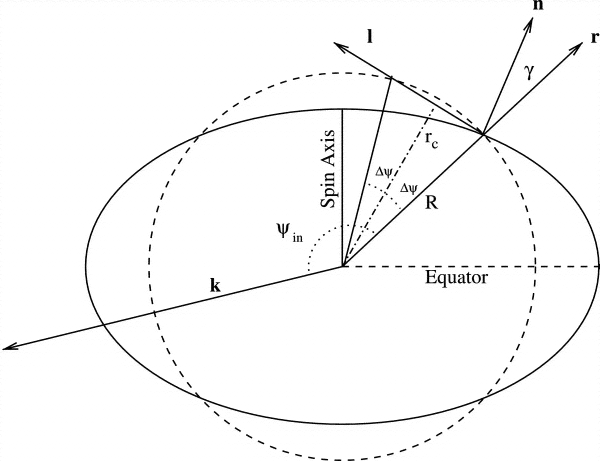
\epsfig{file=oblate_fig.png,width=8.0cm}}
\centerline{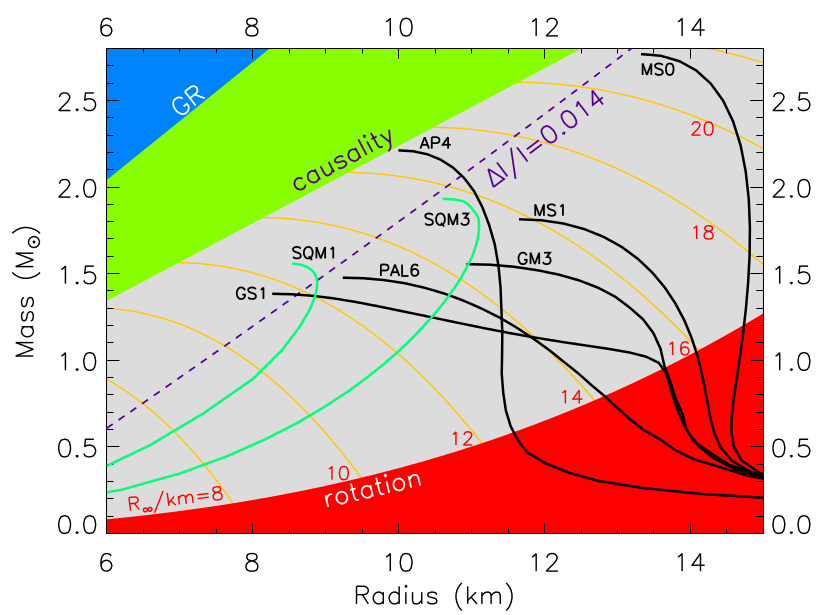
\epsfig{file=eos_mr.png,width=12.0cm}} 
%or maybe lattimer instead
\caption{Mass-radius diagram for neutron stars \cite{lattimer}. Black curves are for normal matter and green curves for SQM equations of state. Regions excluded by general relativity (GR), causality and rotation constraints are indicated. The orange curves shows the contours of constant radiation radii $R_{\infty}$. The dashed line $\Delta I / I = 0.014$ is a limit estimated from the glitches of Vela pulsar \cite{lattimer2001}. Figure 2 from Lattimer and Prakash (2004) \cite{lattimer}.}  
\label{fig:eos_mr}
\end{figure}
%%%%%%%%%%%%%%%%%%%%%%%%%%%%%%%%%%%%%%%%%%%%%











%This is "rhoades":
%http://journals.aps.org/prl/pdf/10.1103/PhysRevLett.32.324 %link works in Tuorla
%Maximum Mass of a Neutron star*
%Clifford E. Rhoades, Jr.,t and Remo Ruffini
%Joseph Henry Iaboratomes, Princeton University, Princeton, Net Jersey 08540
%(Received 30 October 1972)
%On the basis of Einstein's theory of relativity, the principle of causality, and Le Chatelier's
%principle, it is here established that the maximum mass of the equilibrium configuration
%of a neutron star cd~not be larger than 3.2M'. The extremal principle given
%here applies as well when the equation of state of matter is unknown in a limited range of
%densities. The absolute maximum mass of a neutron star provides a decisive method of
%observationally distinguishing neutron stars from black holes.
%One more potential constraint on the EOS is based on the rotation of neutron stars. The velocity of the stellar surface cannot exceed the velocity of an orbiting particle suspended just above the surface ("break-up frequency"). The highest observed spin rate gives a lower limit to the compactness of the neutron star.

%VOLUME 32, NUMBER 6 PHYSICAL R E V I E W L E T T E R S 11 FEBRUARY 1974


\subsection{Accreting millisecond pulsars}




%https://arxiv.org/pdf/1206.2727v4.pdf


Rotating neutron stars were first detected as radio pulsars in 1967 \cite{gold68}. %http://adsabs.harvard.edu/abs/1968Natur.218..731G
After that, many different classes of pulsars have been discovered including low mass X-ray binaries (LMXBs). LMXBs are systems in which the neutron star accretes matter from a non-collapsed companion (with a relatively low mass $M \lesssim  M_{\odot}$) via an accretion disk. Accreting millisecond X-ray pulsars (AMXPs) are a subgroup of the LMXBs, in which the gas from the accretion disk (stripped from the companion) is channeled onto the magnetic poles of a rapidly rotating neutron star. The result is a pair of "hot spots" on the pulsar surface.  This gives rise to the X-ray pulsations with typical periods of a few milliseconds corresponding to the spin frequency of the neutron star. By definition, AMXPs are spinning at frequencies $\nu \ge 100 \, \mathrm{Hz}$ and have weak surface magnetic fields ($B \sim 10^{8-9}$ G) ~\cite{patruno}. A schematic view of the accretion to the hot spots of the pulsar is shown in the figure \ref{fig:shcematic}.


%%%%%%%%%%%%%%%%%%%%%%%%%%%%%%%%%%%%%%%%%%%%%
\begin{figure}
%\centerline{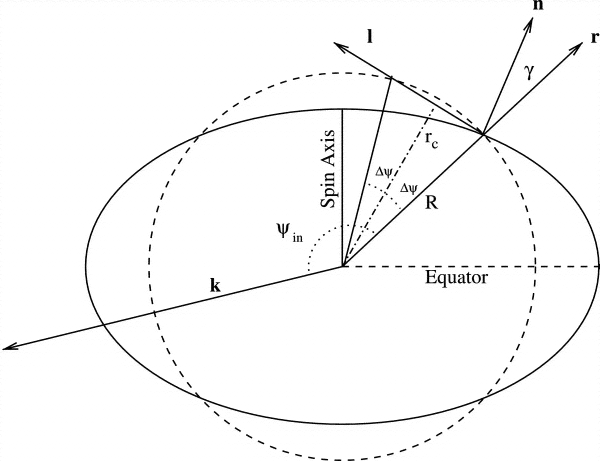
\epsfig{file=oblate_fig.png,width=8.0cm}}
\centerline{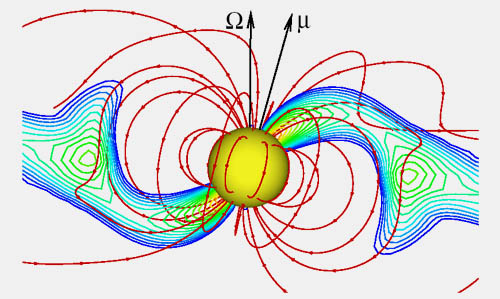
\epsfig{file=schematic.jpg,width=12.0cm}} 
%or maybe lattimer instead
\caption{A view from a magnetohydrodynamical simulation for an accreting compact object with an inclined dipole field. The density of the streaming matter changes exponentially from blue to red. Red lines with arrows show selected magnetic field lines. The magnetic moment, $\bmath{\mu}$, and the rotation axis, $\bmath{\Omega}$, are also shown. Figure 4 from Romanova et. al (2004) \cite{romanova}} 
\label{fig:shcematic}
\end{figure}
%%%%%%%%%%%%%%%%%%%%%%%%%%%%%%%%%%%%%%%%%%%%%
%ROMANOCVA : http://iopscience.iop.org/article/10.1086/421867/pdf

The transfer of mass occurs in all known AMXPs via a Roche lobe overflow from the donor star. The equipotential surface of the binary systems gravitational and centrifugal forces (surrounding the star) is known as Roche lobe. Both the neutron star and the companion have their own lobes that  only join at a inner Lagrangian point $L_{1}$ \cite{frank85}. %http://adsabs.harvard.edu/abs/1985Sci...230.1269F (book in Tuorla)
In the case when the Roche lobe of the companion star is full of matter, the gas left outside the companion's Roche Lobe starts to flow towards neutron star through $L_{1}$. An accretion disk is formed because of the rotation of the system of two stars.
 

The first AMXP discovered was \source. It is also used as a reference target in this thesis. %It is also the main observed target in this thesis. 
The source was first found in 1996 by the Italian-Dutch BeppoSAX satellite \cite{zandsax1808}. %http://adsabs.harvard.edu/abs/1998A%26A...331L..25I
The first coherent pulsations (at 401 Hz) were detected during the second outburst with NASA's Rossi X-ray Timing Explorer (RXTE) in 1998 \cite{wijnandssax1808}. %http://adsabs.harvard.edu/abs/1998Natur.394..344W
It provided a confirmation of the "recycling scenario", which states that AMXPs are the evolutionary progenitors of recycled radio millisecond pulsars. They are responsible for the conversion of slowly rotating neutron stars with high magnetic field ($B \sim 10^{12}$ G), into a rapidly spinning objects with a relatively weak magnetic field ($B \sim 10^{8}$ G) \cite{patruno}. The idea is that a weakening magnetic field allows accretion to happen. The angular momentum of the accreting matter is transferred to the pulsar, which results in the increase of its spin frequency.% of the pulsar.


%SAX J1808.4–3658 went into outburst again in 2000, 2002, 2005, 2008 and 2011,
%with an approximate recurrence time of about 1.6-3.3 yr, and is the best sampled and

After the two first outbursts, \source \ has gone into outburst several times reoccurring approximately every two to three years. It is the best sampled and studied out of all AMXPS. Typically the outburst consists of five phases: a fast rise, with a steep increase in luminosity lasting only a few days, a peak, a slow decay stage, a fast decay phase and the flaring tail. Except the last phase, they are typical for several X-ray binaries and can in principle be partially explained with a so-called instability model (see figure \ref{fig:outburst} for a such outburst).




%%%%%%%%%%%%%%%%%%%%%%%%%%%%%%%%%%%%%%%%%%%%%
\begin{figure}
%\centerline{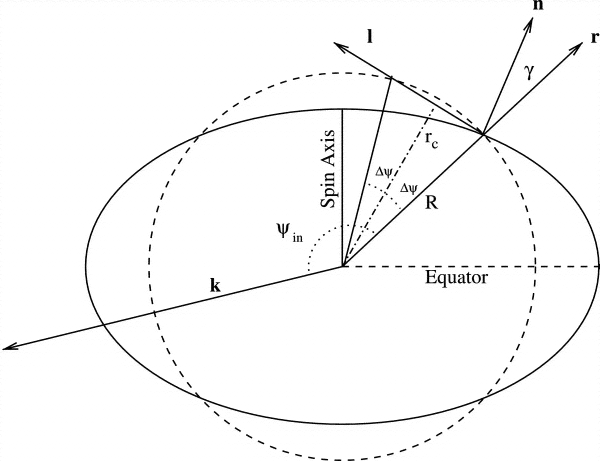
\epsfig{file=oblate_fig.png,width=8.0cm}}
\centerline{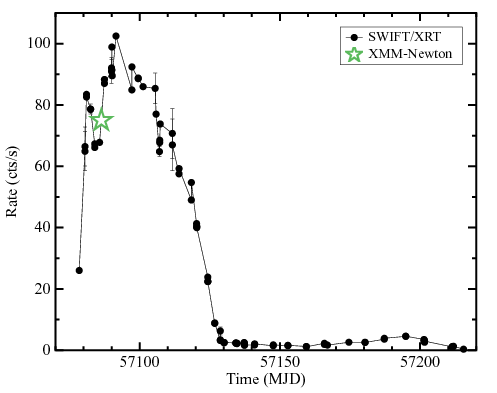
\epsfig{file=outburst.png,width=12.0cm}} 
%or maybe lattimer instead
\caption{Light curve of the 2015 outburst of \sourceb \ as observed by Swift-XRT (black points) and XMM-Newton (the green star). Figure 1 from Sanna et al. (2016) \cite{outburst}.}% The green star represents
%the epoch of the XMM-Newton observation \cite{outburst}.}  
\label{fig:outburst}
\end{figure}
%%%%%%%%%%%%%%%%%%%%%%%%%%%%%%%%%%%%%%%%%%%%%




%The typical outburst can be split in five phases: a
%fast rise, with a steep increase in luminosity lasting only a few days, a peak, a slow
%decay stage, a fast decay phase and the flaring tail. Except the last phase, they can in %principle be partially explained with the disk instability model. 

%pulse profiles from which %phase?


The X-ray spectrum of the outbursts have also been analysed and there is evidence for a two component-model, which includes a blackbody at lower energies and a hard Comptonization component at higher energies \cite{twocompmod} %http://articles.adsabs.harvard.edu/cgi-bin/nph-iarticle_query?2002MNRAS.331..141G&defaultprint=YES&filetype=.pdf]
. The heated hot spot on the neutron star surface is interpreted to produce the blackbody flux. The Comptonization is produced above the spot in a accretion shock. This shock is created as the plasma abruptly decelerates close to the neutron star surface at the bottom of the magnetic field lines.



\iffalse

The RXTE observatory has played an extraordinary role by discovering many
systems of this kind and by collecting extensive data records of each outburst detected
during its fifteen year lifetime. The excellent timing capabilities of RXTE
have brought new means to study NSs with coherent X-ray timing, and helped to
constrain the long term properties of many AMXPs over a baseline of more than
a decade. Observation of the orbital Doppler shift of the AMXP pulse frequency
contains information on the orbital parameters of the binary and their evolution in
time. Binary evolution has benefited from the study of AMXPs [13, 14, 15] which

are now known to include ultra-compact systems (orbital period Pb . 80 min) with
white dwarf companions, compact systems (Pb ≃ 1.5 − 3 hr) with brown dwarf
donors and wider systems (Pb ≃ 3.5 − 20 hr) with main sequence stars. Other Xray
and gamma ray space missions like XMM-Newton, INTEGRAL, Chandra, Swift
and HETE have also played an important role in discovering and understanding the
spectral and timing properties of these objects. Multiwavelength observations covering
radio, infrared, optical and UV wavelengths have also illuminated different
aspects of these fascinating systems. Several optical and infrared counterparts have
been identified with ground based observations and in some cases have led to the
discovery of the spectral type of the donor, while radio and infrared observations
have revealed the possible presence of jets.

\fi

\clearpage

\section{Methods}

%There have been many different attempts to constrain the masses and radii of neutron stars and thus also the possible equations of state. For example one approach is the so called cooling tail method, where the observed cooling tracks of thermonuclear X-ray bursts are compared to the accurate theoretical atmosphere model calculations \cite{nattila_bayes}. One other approach to measure $M$ and $R$ is to fit detailed spectral models to high-precision measurements of X-ray burst spectra \cite{madej}. %http://adsabs.harvard.edu/abs/2005AcA....55..349M
%This however requires very high-precision spectral data. 

There have been many different attempts to constrain the masses and radii of neutron stars and thus also the possible equations of state. The approach we use here is to fit a pulse profile model to the observed X-ray oscillations of accretion-powered millisecond pulsars. In this section we first present our waveform model and then the Bayesian methods we use to get constraints for the parameters of the model. %The final aim is to combine constraints obtained with different approaches.

\subsection{Pulse profile modeling}


The oscillations in the flux during the outbursts (the light curves) of accreting millisecond pulsars (described in the first chapter) can be modeled with different models. The model presented here assumes that the radiation is originated from one or two of the polar caps of the star. General and special relativistic effects have been taken account using so-called Schwarzschild-Doppler (S+D) approximation %(Miller, Lamb 1998   
\cite{millerlamb98}%http://adsabs.harvard.edu/abs/1998ApJ...499L..37M
%, Poutanen, Gierlinski 2003 
\cite{poutagierlinskisax}. In the S+D approximation the effects of general relativity (gravitational light-bending) are modeled as though the star is not rotating using the Schwarzschild metric and the formalism specified by
Pechenick, Ftaclas and Cohen (1983) \cite{pechenick}. Rotational effects have been approximated by using special relativistic Doppler transformations as though the star is a rotating object with no gravitational field. The oblate shape of the rapidly rotating neutron stars have also been taken account using an empirical formula for the oblate shape.

%Rotational effects are added by introducing Doppler terms as though the star is a rotating object with no gravitational field. The oblate shape of the rapidly rotating neutron stars have also been taken account using an empirical formula for the oblate shape.

The observed pulse profiles from AMXPs appear to be rather close to sinusoidal with peak-to-peak oscillation amplitude 
\be \label{eq:amplitude}
A = \frac{F_{\mathrm{max}} - F_{\mathrm{min}}} {F_{\mathrm{max}} - F_{\mathrm{min}}}
\ee %https://arxiv.org/pdf/astro-ph/0510038v2.pdf
 between 4 and 12 per cent \cite{poutarew2006}, where $F_{\mathrm{max}}$ is the maximum observed flux and $F_{\mathrm{min}}$ is the minimum observed flux. Light bending tend %error, where?
to reduce the variability amplitude. The amplitude depends only weakly on energy and the spectrum may be fitted with a two-component model (blackbody and Comptonization). At higher energies the amplitude deviate more from a sine wave because of the different emission pattern. The weak energy dependency and a fairly constant spectral shape as a function of pulse phase, support also the idea that the bulk of the observed X-ray emission originates from polar caps (where the gas stream channeled by the neutron star magnetic field impacts the stellar surface forming a shock). Any additional source of radiation would have to have a spectrum identical to that of the shock.


\subsubsection{Oblateness}

Due to the fast rotation the millisecond pulsars have an oblate shape instead of spherical. The difference between an oblate and a spherical star is significant when the rotation frequency $\nu \ge 300 \, \mathrm{Hz}$ \cite{cadeau}%a place for a reference..
. The most important effect is purely geometrical: The directions that the light can be emitted into are different in the cases of an oblate and a spherical star. Thus there are certain spot locations on the star where the spot is invisible if the surface is oblate but would be visible if the surface were spherical (and vice versa).


There are different models describing the exact shape and oblateness of the neutron star (function $R(\theta)$, where $\theta$ is the colatitude measured from the spin axis).
%The exact shape and oblateness of the star (function $R(\theta)$) can be chosen from different models ($\theta$ is the colatitude measured from the spin axis).
One of the most recent ones was presented by Algendy et. al. (2014) \cite{algendy}. 
It is also the model we use primarily in this thesis. In that model (in geometric units
where G = c = 1)

\begin{equation}
\label{rtheta2}
\frac{R(\theta)}{R_{\mathrm{eq}}} = (1 + o_{2}(x,\bar{\Omega})\cos^{2}(\theta)),
\end{equation}
where


\begin{equation}
\label{otwo}
o_{2}(x,\bar{\Omega}) = \bar{\Omega}^{2}(-0.788+1.030x),
\end{equation}


\begin{equation}
\label{rtheta2x}
x = \frac{M}{R_{\mathrm{eq}}},
\end{equation}


\begin{equation}
\label{rtheta2omega}
\bar{\Omega} = \Omega (\frac{R_{\mathrm{eq}}^{3}}{M})^{1/2}.
\end{equation}


In these equations $R_{\mathrm{eq}}$ is the radius of the rotating star measured at the equator and $\Omega = 2\pi/P$, where P is the spin period. The equator radius is measured in the normal Schwarzschild coordinates as all the radii are in this thesis.

One other model we have also used in pulse profile comparison was presented by Morsink et al. (2007) \cite{morsink}. In that model


\be\label{eq:rtheta}
\frac{R(\theta)}{R_{eq}} = 1 + \sum\limits_{n=0}^2 a_{2n}(\zeta_{0},\epsilon_{0})P_{2n}(\cos(\theta)), 
\ee
where $P_{n}(\cos(\theta))$ is the Legendre polynomial of order $n$ and parameters $\zeta_{0}$ and $\epsilon_{0}$ are obtained from

\be\label{eq:parzeta}
\zeta_{0} = \frac{GM}{R_{eq}c^{2}}
\ee

\be\label{eq:parepsilon}
\epsilon_{0} = \frac{\Omega^{2}R_{eq}^{3}}{GM}.
\ee
The coefficients needed are given as

\be\label{eq:azero}
a_{0} = -0.18\epsilon_{0}+0.23\zeta_{0}\epsilon_{0}-0.05\epsilon_{0}^{2} 
\ee

\be\label{eq:atwo}
a_{2} = -0.39\epsilon_{0}+0.29\zeta_{0}\epsilon_{0}+0.13\epsilon_{0}^{2}
\ee

\be\label{eq:afour}
a_{4} = +0.04\epsilon_{0}-0.15\zeta_{0}\epsilon_{0}+0.07\epsilon_{0}^{2}.
\ee


\subsubsection{Geometry}

Besides the geometry of the star itself, we also need to know the relations between different angles in different frames. To derive these we consider a small spot on the stellar surface at colatitude $\theta$ from the rotational pole (we follow closely the derivation of Poutanen and Beloborodov (2006) \cite{poutabelo}). 
The star is assumed to be rotating  with a frequency $\nu=P^{-1}$ (seen by a distant observer).
The velocity of the spot in units of $c$ (as measured by an non-rotating observer near the star)  %<- correct now?
is 
\begin{equation}
\label{beta2}
\beta = \frac{v}{c}=\frac{2\pi R(\theta)}{c} \frac{\nu}{\sqrt{1-u}} \sin\theta =\beta_{\rm eq}(\theta) \sin\theta,
\end{equation}
where $\beta_{\rm eq}$ would be constant if the star were spherical, $u\equiv\rg/R(\theta)$, 
$\rg=2GM/c^2$ is the Schwarzschild radius, $M$ is mass and $R(\theta)$ is
radius of the star at spot location (given by equation \ref{rtheta2}). The pulsar frequency has been corrected for the gravitational redshift $1/\sqrt{1-u}=1+z$, since the rotation frequency seen by distant observer is reduced in the gravitational field of the star due to the gravitational time dilation. The corresponding Lorentz factor for the velocity of the spot is $\Gamma=(1-\beta^2)^{-1/2}$.

Because of the fast rotation and special relativistic effects, spot area $\d S^\prime$ measured in a corotating frame is not same as the area $\d S$ measured in a non-rotating frame. The instantaneous position of the spot in the fixed lab frame is described by the unit vector 
\begin{equation}
\bmath{r}=(\sin\theta\cos\phi, \sin\theta\sin\phi, \cos\theta),
\end{equation}
that points to the spot from the center of the star (see Fig. ~\ref{fig:geom2}). The rotational phase of the pulsar is $\phi=2\pi\nu t$. The vector $\bmath{r}$ is not usually directed perpendicular to the surface of the spot unless if the star is spherical. The vector that points normal to the surface is given by
\begin{equation}
\bmath{n}=(\sin(\theta-\gamma)\cos\phi, \sin(\theta-\gamma)\sin\phi, \cos(\theta-\gamma)).
\end{equation}
The angle between $\bmath{n}$ and $\bmath{r}$ is $\gamma$ and 
\begin{equation}
\cos\gamma=[1+f^{2}(\theta)]^{-1/2},
\end{equation}
where
\be \label{eq:ftheta}
f(\theta)=\frac{1+z}{R}\frac{dR}{d\theta}.
\ee
In case of a spherical star $\frac{dR}{d\theta} = 0$ and thus $\bmath{n} = \bmath{r}$.

%%%%%%%%%%%%%%%%%%%%%%%%%%%%%%%%%%%%%%%%%%%%%
\begin{figure}
%\centerline{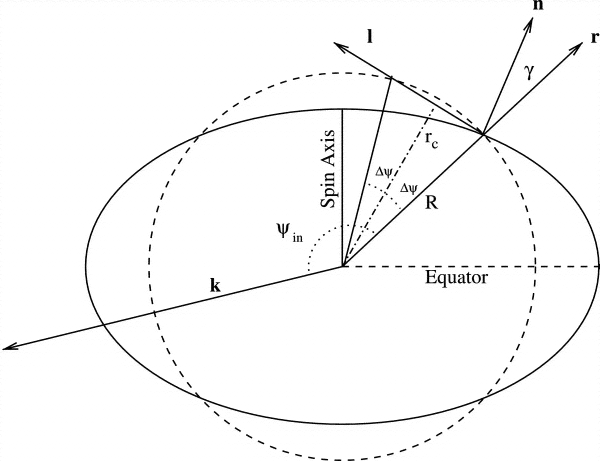
\epsfig{file=oblate_fig.png,width=8.0cm}}
\centerline{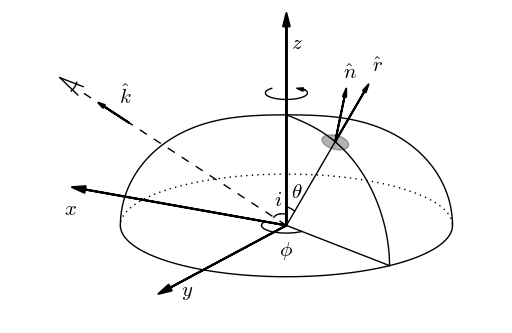
\epsfig{file=fig2.png,width=12.0cm}}
\caption{Geometry of the problem. Created with https://github.com/natj/nsfig. %Dotted curve shows a spherical star which radius is equal to the radius of the oblate star at spot location (\cite{morsink}).%Dotted curve shows the
%photon trajectory.
\label{fig:geom2}}
\end{figure}
%%%%%%%%%%%%%%%%%%%%%%%%%%%%%%%%%%%%%%%%%%%%%



%We will start the waveform with the center of the spot in the plane defined... 
The computation of the waveform is started from the center of the spot in the plane defined by the spin axis and the direction to the observer 
(when the spot crosses the plane defined by $\bmath{z}$ and $\bmath{k}$). The light pulse originating at this moment at the point that is directly below the observer and with a reference distance to the center of the star (e.g., the equator radius of the star) is used to define the zero of the observer's time coordinate. Measuring of the time $t$ is started when this photon arrives at the observer (hence fixing $t=0$). %The time is set to zero when this photon arrives at the observer. 



We denote the unit vector along the line of sight by 
\be
\bmath{k}=(\sin i, 0, \cos i), 
\ee 
where $i$ is the inclination angle of the spin axis to the line of sight. 
Thus (see Fig. \ref{fig:geom2})
\be \label{eq:psi2}
  \cos\psi=\bmath{k}\cdot \bmath{r} = \cos i\ \cos\theta+\sin i\ \sin \theta\ \cos\phi,
\ee

The lensing angle $\psi$ measures the angle between the line of sight and the position vector $\bmath{r}$ of the spot. The initial angle of the emitted photon with respect to
 ${\mathbf r}$ differs from $\psi$ because of the light bending.

%Angle $\psi$ measures the apparent inclination of the spot to the line of
%sight, which is different from the true inclination because of
%the light bending effect. %IS THIS CORRECT?


% The initial angle of the emitted photon with respect to the normal
% ${\mathbf n}$ differs from $\psi$ because of the light bending.
We denote the initial direction of the emitted photon by $\bmath{k}_0$ %($\bmath{l}$ in figure \ref{fig:geom2})
and the true emission angle (relative to $\bmath{r}$) by $\alpha$, so that
\be
 \cos\alpha=\bmath{k}_0 \cdot \bmath{r}.
\ee
The zenith angle $\sigma$ between the $\bmath{n}$ and $\bmath{k_{0}}$ is defined by 
\be
\cos\sigma = \bmath{k_{0}}\cdot\bmath{n}.
\ee

The direction of the photon changes from $\bmath{k}_0$ near the stellar surface to $\bmath{k}$ at infinity as it propagates to infinity, so that $\cos\alpha=\bmath{k}_0\cdot\bmath{r}$
changes to $\cos\psi=\bmath{k}\cdot\bmath{r}$.
%As a photon propagates to infinity, its direction changes from
%$\bmath{k}_0$ near the stellar surface to $\bmath{k}$ at infinity,
%so that $\cos\alpha=\bmath{k}_0\cdot\bmath{r}$
%changes to $\cos\psi=\bmath{k}\cdot\bmath{r}$.
The relation between $\bmath{k}_0$ and $\bmath{k}$ may be written as
\be\label{eq:k02}
\bmath{k}_0=[ \sin\alpha\ \bmath{k} +\sin(\psi-\alpha)\ \bmath{r}]/\sin\psi.
\ee
%At any moment of time, we can introduce an instantaneous non-rotating frame $x,y,z$ 
%with the $y$-axis along the direction of the spot motion, 
%$x$-axis along the meridian towards the equator, and 
%$z$-axis along the normal  to the spot.
%In this static frame
We would like to express this vector in the rest frame of the spot instead of the non-rotating static frame. As a first step we do the coordinate transformation to an instantaneous non-rotating frame $x,y,z$ with the $y$-axis along the direction of the spot motion, $x$-axis along the meridian towards the equator, and $z$-axis along the normal of the spot. This frame can be introduced in any moment of time. In this static frame
\be 
\bmath{k}_0=
\left( 
%\frac{\sin\alpha}{\sin\psi} (\sin i\cos\theta\cos\phi -\cos i \sin\theta),
\cos \epsilon,
\cos\xi, 
\cos\sigma
\right) ,
\ee 
where $\xi$ is the angle  between the spot velocity and the direction of the emitted photon $\bmath{k}_0$. It is given as   
\be \label{eq:cosxi22}
\cos\xi=\frac{\bmath{\beta}}{\beta} \cdot \bmath{k}_0
=\frac{\sin\alpha}{\sin\psi} \frac{\bmath{\beta}}{\beta} \cdot \bmath{k}=
- \frac{\sin\alpha}{\sin\psi}\sin i\ \sin\phi\ ,
\ee
since $\bmath{\beta} = \beta(-\sin\phi,\cos\phi,0)$ in the lab frame. Angle between the meridian % And $\epsilon$ is the angle between the meridian 
\be
 \bmath{m} = (\cos(\theta - \gamma)\cos \phi ,\cos (\theta -\gamma)\sin \phi, -\sin (\theta -\gamma))
\ee
and $\bmath{k}_0$ is $\epsilon$, which is obtained from 

\be \label{eq:kx-comp}
\begin{split}
\cos\epsilon= \bmath{m} \cdot \bmath{k}_0
=\frac{\sin\alpha}{\sin\psi} (\sin i \cos(\theta -\gamma)\cos \phi -\cos i \sin (\theta -\gamma)) \\ + \frac{\sin (\psi - \alpha)}{\sin \psi}(\sin \theta \cos (\theta -\gamma)-\sin (\theta -\gamma)\cos \theta).
\end{split}
\ee

%But also $\bmath{\beta}$ (y-axis) and $\bmath{n}$ (z-axis)should be perpendicular???? Okey, I think it is both same time .. +if you choose $\bmath{r}$ as z-axis, then the z-component of $\bmath{k_{0}}$ will be $\cos\alpha$)

Next we can consider a frame which have the same axes as previously but which is also corotating with the spot. We want to express the direction of the emitted light also in this frame. Emission angle relative to the surface normal in this frame is denoted by
$\sigma'$.  It differs from $\sigma$ because of relativistic aberration. The rays of light are tilted towards the direction of the spot motion relative to the observer.
In this frame comoving with the spot 
(with $y$-axis again along the spot motion and $z$-axis along the local normal), 
the unit vector along the photon momentum  is 
obtained from the Lorentz transformation: 
\be \label{eq:k0prime2}
\bmath{k}'_0 = \Dop
\left( \begin{array}{c}
%(\sin i\cos\theta\cos\phi -\cos i \sin\theta)\sin\alpha/\sin\psi \\
\cos \epsilon \\
\Gamma (\cos\xi-\beta)\\ 
\cos\sigma
\end{array}
\right) ,
\ee 
where $\delta$ is the Doppler factor formulated as
\be \label{eq:dop2}
\Dop=\frac{1}{\Gamma(1-\beta\cos\xi)} .
\ee
Using equation (\ref{eq:k0prime2}), we obtain
\be \label{eq:aberr2}
\cos\sigma' =   \Dop \ \cos\sigma ,
\ee
 
Making use of equation (\ref{eq:k02}) the zenith angle has the value
\be\label{eq:cossigma2}
\begin{split}
\cos\sigma = \bmath{k_{0}}\cdot\bmath{n} = \cos\alpha\cos\gamma+\sin\alpha\sin\gamma\cos\zeta = \\
\cos \alpha  \cos \gamma + \frac{\sin \alpha}{\sin \psi} \sin \gamma (\cos i \sin \theta - \sin i \cos \theta \cos \phi),
\end{split}
\ee
where the spherical trigonometric identity $\cos i = \cos\theta\cos\psi+\sin\theta\sin\psi\cos\zeta$ (where $\zeta$ is the angle between the spot-observer and the spot-spin-axis planes) and the equation (\ref{eq:psi2}) are used. With small bending angles the approximation $\frac{\sin \alpha}{\sin \psi} \approx \sqrt{(1-u)}$ may be used. This is based on the Beloborodov's approximation  \cite{beloborodov}
\be \label{eq:beloborodov}
1-\cos \alpha = (1 - \cos \psi)(1 - u).
\ee
%if $\sin\psi\sin\theta \ne 0$. If $\sin\psi\sin\theta = 0$, then $\cos\sigma = \cos\alpha\cos\gamma$.
The equation (\ref{eq:cossigma2}) is useful, since we need to know the emission angle relative to the spot normal ($\sigma$) in order to calculate fluxes and visibility conditions. 


\subsubsection{Light bending}

Before we can get the angle $\sigma$ from equation (\ref{eq:cossigma2}) we also first need to know how to get the angle $\alpha$ when we know the light bending angle $\psi$. The angles $\psi$ we know (for every point at every phase) directly from the geometry, since we can calculate them using the equation (\ref{eq:psi2}). In case of non-infinitesimal spot (which is discussed more in the Section 2.1.6) we of course need a  transformation of coordinates between the spot frame and the frame of the star (to get corresponding $\theta$ and $\phi$ for every point inside the spot). The angle $\psi$ is anyway straight determined, since we are going to calculate the trajectories for only those photons which are going to arrive at the observer (not in some other direction). The task is now to find out the true emission angle $\alpha$ using general relativity. 

The exact relation between $\alpha$ and $\psi$ (when $\alpha < \pi/2$) in Schwarzschild geometry (i.e. light bending) is given by \cite{mtw}%(e.g. Misner et al. 1973 \cite{mtw}) %\citep[e.g.][]{mtw73}
\be \label{eq:bend2}
  \psi_{p}(R,\alpha)=\int_R^{\infty} \frac{dr}{r^2} \left[ \frac{1}{b^2} -
       \frac{1}{r^2}\left( 1- \frac{\rg}{r}\right)\right]^{-1/2} ,
\ee
where $b$ is the impact parameter,
\be \label{eq:impact2}
  b=\frac{R}{\sqrt{1-u}} \sin\alpha .
\ee
The relation between  $\alpha$ and $\psi$, when $\alpha > \pi/2$, is 
\be 
\psi(R,\alpha)=2\psi_{\max}-\psi_{p}(R,\pi-\alpha),
\ee 
where $\psi_{\max} = \psi_{p}(p,\alpha=\pi/2)$ and $p$ is the distance of closest approach, given by
\be
p = -\frac{2}{\sqrt{3}}b\cos([\arccos(3\sqrt{3}\rg/(2b))+2\pi]/3).
\ee


Numerical calculations using directly integral (\ref{eq:bend2}) lead to dramatic errors, but after making a variable substitution $x = \sqrt{1-R/r}$ the integral can be computed without problems using for example Simpson quadratures. Even though it is not possible to obtain $\alpha$ as an exact function of $\psi$, we can still use the previous equations to form a two-dimensional grid of $\psi$ corresponding to different $\alpha$ and $R$. Then we find the correct $\alpha$ at different phases of the rotation of the star by quadratic interpolation. 



The maximum bending angle corresponds to $\sigma=\pi/2$. Otherwise the photon would be directed across the star surface. 
The condition $\cos \sigma>0$ is used to define the visibility of the spot. In addition one should also check that the photon won't hit the surface of the star in any later phase of its trajectory (it might happen for an oblate star). This check is not yet included in the current pulse profile code.


\subsubsection{Observed flux}

Next we can consider the flux originating from our small spot. The observed flux from the spot at photon energy $E$ is
\be
\label{eq:dF_E2}
  \d F_E=I_E\ \d\Omega,
\ee
where $I_E$ is the specific intensity of radiation at infinity and $\d\Omega$ is
the solid angle covered by the spot (with area $\d S'$ in the corotating frame) on the observer's sky.
The solid angle can be expressed in terms of the impact parameter \cite{pechenick}
\be
\d\Omega=b\ \d b\ \d\varphi/D^2,
\ee
where $D$ is the distance to the source and $\varphi$ is the azimuthal
angle corresponding to rotation around line of sight (vector $\bmath{k}$).
The impact parameter $b$ depends only on the bending angle $\psi$, but not on $\varphi$.

%The apparent area of the spot as measured by photon beams
%in the non-rotating frame near the stellar surface is $\d S=\Dop\ \d S'$

The apparent area of the infinitesimal spot measured by the observer in the non-rotating frame near the stellar surface %(but also at infinity) %not true? .. note: dS*cos(sigma) = Lorentz invariant
is $\d S=\Dop\ \d S'$ \cite{terrell}\cite{lightman75}.
%(see Terrell 1959 \cite{terrell} or Lightman et al. 1975 \cite{lightman75}). %; Ghisellini 1999) %http://journals.aps.org/pr/pdf/10.1103/PhysRev.116.1041 (terrell)
%lightman75 = problem book in relativity and gravitation (found in Tuorla)
%didin't found $\d S=\Dop\ \d S'$
We also know the relation between $\sigma$ and $\sigma'$ from the relativistic aberration formula \ref{eq:aberr2} (for motions parallel to the spot surface) $\cos\sigma' =   \Dop \ \cos\sigma$. Thus 
\be \label{eq:Salpha2}
\d S\ \cos\sigma = \d S'\ \cos\sigma', 
\ee
which shows that the spot area projected on to the plane perpendicular to the photon direction is Lorentz invariant \cite{lightman75}\cite{lindbland85}%(see e.g.  Lightman et al. 1975 \cite{lightman75} or 
%Problem book in relativity and gravitation
%Lind \& Blandford 1985 \cite{lindbland85}). 
This area is also called a photon beam cross-section.
The infinitesimal spot area measured in the frame comoving with the spot may be calculated as \cite{morsink} %(Morsink et al. 2007 \cite{morsink})
\be \label{eq:surf_element}
\d S'(\theta) = R^{2}(\theta) [1+f^{2}(\theta)]^{1/2} \sin \theta \d \theta \d \phi,
\ee
where the factor $[1+f^{2}(\theta)]^{1/2}$ takes into account the oblateness of the spot surface (function $f(\theta)$ is given in equation \ref{eq:ftheta}).
%which shows that the spot area projected on to the plane perpendicular 
%to the photon propagation direction, i.e. a photon beam cross-section,
%is Lorentz invariant (see e.g.  Lightman et al. 1975 \cite{lightman75} or %Problem book in %relativity and gravitation
%Lind \& Blandford 1985 \cite{lindbland85}). 
%Using equation~(\ref{eq:impact2}) and
%the facts that $\d S=R^2\ \d\cos\psi\  \d\varphi$  (THIS IS NOT CORRECT %NOW) one gets... (see Morsink)
The solid angle measured at a distance $D$ from the star is then \cite{morsink}
\be\label{eq:omega2}
 \d\Omega=\frac{\d S' \cos \sigma'}{D^2} \frac{1}{1-u} \frac{\d\cos\alpha}{\d\cos\psi}.
\ee
In case of stars with lower compactness (weak gravity) $\rg \ll R$, so $u\ll 1$, and this gives
the usual formula $\d\Omega=\d S' \cos \sigma'/D^2$. 

%The combined effect of the gravitational redshift and Doppler effect
%results in the following  relation between the monochromatic
%observed and local intensities

We have now obtained the solid angle $\d\Omega$ needed to calculate the flux from our spot with equation (\ref{eq:dF_E2}). However we still need to find out a expression for intensity $I_{E}$. The intensity is also different in the static frame of the distant observer than in the local frame comoving with the spot due to both gravitational redshift and Doppler effect. The relation between monochromatic observed and local intensities is \cite{mtw}\cite{rybicki}%(see e.g. Misner et. al. 1973 \cite{mtw} or Rybicki \& Lightman 1979 \cite{rybicki})%\citep[see e.g.][]{mtw73,rl79}:
\be
I_{E} = \left (\frac{E}{E'}\right )^3 I'_{E '} (\sigma')
\ee
where $E/E'=\Dop \sqrt{1-u}$. Here $I'_{E'}(\sigma')$ is the intensity computed in the corotating frame. The dependence of redshift ($1+z = 1/\sqrt{1-u}$) to the power of 3 can be understood by noting that $I_{E} \propto \nu^{3}$ and $\nu = \nu'(1+z)^{-1}$.
For the bolometric intensity the dependence on frequency goes to $\nu^{4}$ and one gets
\be \label{eq:bolointensity}
I= \left (\Dop \sqrt{1-u} \right )^4 I'(\sigma') .
\ee

The observed spectral flux (eq.~\ref{eq:dF_E2}) is now given by
\be \label{eq:fluxspot2}
\d F_{E}=(1-u)^{1/2} \Dop^{4} I'_{E'}(\sigma') \cos\sigma
\frac{\d \cos\alpha}{\d\cos\psi}
 \frac{\d S'}{D^2} ,
\ee
where we have used the aberration formula (\ref{eq:aberr2}).
The bolometric flux reads:
\be  \label{eq:fluxbolo2}
\d F= (1-u)\ \Dop^5 \
I'(\sigma')  \cos\sigma \frac{\d\cos\alpha}{\d\cos\psi} \frac{\d S'}{D^2} .
\ee
The radiation spectrum can be e.g., a blackbody, with effective temperature $T_{\mathrm{eff}}$ or a power-law spectrum. We can take for example a power-law $I'_{E'}(\sigma') \propto E '^{-(\lambda-1)}$, which does not depend on the angle $\sigma'$. Here $\lambda$ is the photon spectral index. With this spectrum we get
\be \label{eq:int_trans2}
I'_{E'}(\sigma') = I'_{E}(\sigma')
\left( \Dop \sqrt{1-u} \right)^{\lambda-1} .
\ee
The observed spectral flux %at a distance $D$ from the star 
may be then expressed as
\be\label{eq:fluxplaw2}
\d F_{E}= (1-u)^{\lambda/2}\ \Dop^{\lambda+3} I'_E(\sigma')
\cos\sigma\ \frac{\d\cos\alpha}{\d\cos\psi}\ \frac{\d S'}{D^2}.
\ee
We note that the equation for the bolometric flux (\ref{eq:fluxbolo2})
can be obtained as a special case of Eq.~(\ref{eq:fluxplaw2}) by setting $\lambda=2$. 

Let us look the expression (\ref{eq:fluxbolo2}) for the bolometric flux more carefully. We see that there is a difference by a factor $\Dop^5$ between the flux from a rapidly rotating star and that from a slowly rotating star. One power of the Doppler factor came from the change in the projected area due to aberration as we already mentioned. From the four other powers of Doppler factor (appearing in the equation \ref{eq:bolointensity}) two comes from the solid angle transformation, one from the energy and one from the time contraction of photon arrival \cite{rybicki}. %(Rybicki \& Lightman 1979 \cite{rybicki}). 
In the case of spectral flux (equation \ref{eq:fluxspot2}) there is no Doppler factor from the energy and thus there is one power less.


%Two powers of $\Dop$ come
%from the solid angle transformation, one from the energy, one from the
%photon arrival time contraction,
%and the fifth from the change in the projected  area due to  aberration.
%Aberration may also change the specific intensity since it has to be computed
%for angle $\sigma'$ in the comoving frame. 

As mentioned, in the most simple model we may assume that the intensity is independent of $\sigma'$ ("isotropic beaming"). In a little more general case one can assume the intensity to be a product of an angle-dependent ("beaming function") and an energy-dependent function. The beaming function describes how much intensity is emitted to each direction and the function might have e.g., a polynomial shape. An atmosphere dominated by electron scattering produces a beaming function called Hopf profile, which is approximately polynomial.  


Thanks to the observed AMXPs (e.g., \source \ \cite{poutagierlinskisax}) we know that the spectrum of the pulsar (i.e., the energy-dependence of $I'_{E'}(\sigma')$ ) might be fitted with a blackbody component at lower energies and with a power-law component at higher energies. However in the case of \source \ the blackbody contributes only about 30 per cent to the flux even in the 3-5 keV region (which is near the lowest observed energies with RXTE) \cite{poutagierlinskisax}. Thus we can approximate the spectrum with two different power-laws on both sides of a cut-off energy, which is defined to be at the maximum flux of a blackbody with $T_{\mathrm{eff}} = 2 $ keV (in the frame of the spot). Below the cut-off energy we use Rayleigh-Jeans law ($I'_{E'}(\sigma') \propto E '^{2}$ and thus $\lambda = -1$) and above the cut-off a descending power-law with the spectral index $\lambda = 1.86$. The power-law is normalized to be equal with the reference blackbody at 1 keV. This spectrum is shown in the Figure \ref{fig:spectrum}.


%%%%%%%%%%%%%%%%%%%%%%%%%%%%%%%%%%%%%%%%%%%%%
\begin{figure}
\centerline{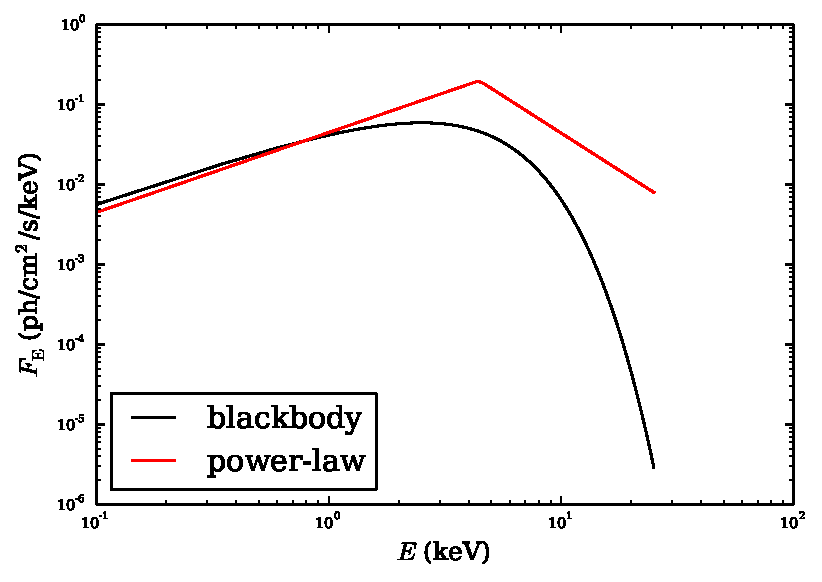
\epsfig{file=spectrum_numflux0.pdf,width=12.0cm}}
\caption{The two-component power-law compared to a blackbody at 2 keV temperature. The spectra are calculated using the time-averaged fluxes at different energies of the pulse profile model with some physical parameters. 
\label{fig:spectrum}}
\end{figure}
%%%%%%%%%%%%%%%%%%%%%%%%%%%%%%%%%%%%%%%%%%%%%


In a more realistic model we would calculate the fluxes using two overlapping spots. The other spot would produce blackbody emission with isotropic beaming and the other one the power-law emission with e.g., a linear dependence on the beaming angle $\sigma'$ (representing the accretion shock). The spots may have different shapes and sizes. %This model will be added to the pulse profile code in the near future.


In the calculations of this thesis we use monochromatic number fluxes (in units of photons/cm$^{2}$/s/erg), since those are the fluxes we get from the observations. We must thus divide the fluxes we get from equation (\ref{eq:fluxspot2}) with the observed energy $E$. When calculating the flux we make again a grid of values of the derivatives $\frac{\d\cos\psi}{\d\cos\alpha}$ (same as $(\frac{\d\cos\alpha}{\d\cos\psi})^{-1}$) with different $\alpha$ and $R$. The derivatives for each point are found by linear interpolation. 


\subsubsection{Time delays}



The previous expressions (\ref{eq:fluxspot2}), (\ref{eq:fluxbolo2}) and (\ref{eq:fluxplaw2}) for calculating the flux of an infinitesimal spot
contain the pulsar phase $\phi$ expressed in $\cos\sigma$. However we should realize that photons are not necessarily observed in the same order as they are emitted due to the different light travel times when the position of the emitting spot is different. For this reason the flux actually corresponds to an observed phase $\phiobs$, which is different from $\phi$. The delays between light travel times become significant only for rapidly rotating pulsars. %In Schwarzschild metric the maximum time delay for a neutron star
%of $M=1.4\msun$ is $\Delta t\sim 7\times 10^{-2}$ ms (almost independent
%of compactness of the star $M/R$). This gives at most 
%a 5 per cent correction to the arrival phase for a rotational period $P=1.5$~ms.
%citate here to JP pulse profile comparisons paper?

   
%The delay is caused by different travel times of emitted
%photons to the observer, depending on the position of the emitting spot.

The different light travel times in Schwarzschild metric may be calculated and subtracted to get the time delay between the photon from the point of interest and a photon from a reference point (we call this the reference photon). We choose the reference point to locate at a reference radius $r_{\mathrm{ref}}$ from the center of the star (it can be chosen arbitrarily as long as it exceeds $\rg$) and assume that the reference photon is emitted exactly to the radial direction (meaning that $\alpha$ = 0 and thus impact parameter $b = 0$). Now a photon following the trajectory with an impact parameter $b$ (and $\alpha < \pi/2$) is lagging the reference photon by 
%A photon following the trajectory with an impact parameter $b$ (and $\alpha < \pi/2$)
%is lagging the photon originating from a reference radius $r_{\mathrm{ref}}$ (which %can be chosen arbitrarily as long as it exceeds $\rg$) with $b=0$ by 
%(Pechenick et al. \cite{pechenick})%\citep{pfc83}:
%:
\cite{pechenick}
\be \label{eq:delay2}
c\Delta t_{p}(R,\alpha)=  c\Delta t_{s}(R,\alpha) -\delta t(r_{\mathrm{ref}},R),
\ee
where 
\be \label{eq:delayint}
c\Delta t_{s}(R,\alpha) =
\int_R^{\infty} \frac{\d r}{1- \rg/r}
\left\{ \left[ 1-  \frac{b^2}{r^2}  \left( 1- \frac{\rg}{r} \right)
\right] ^{-1/2}  -1 \right\}
\ee
is the time difference between photons originating from the same radius $R$ and
\be
\delta t(r_{\mathrm{ref}},R) = R-r_{\mathrm{ref}}+\rg\ln(\frac{R-\rg}{r_{\mathrm{ref}}-\rg})
\ee
is the time difference between photons with $b=0$ from $R$ and $r_{\mathrm{ref}}$ \cite{falkner}. 
%%(...) Citate here to falkner

In the case when $\alpha > \pi/2$ the corresponding delay is
\be\label{eq:delay22}
\begin{split}
c\Delta t(R,\alpha)= 2c\Delta t_{s}(p,\pi/2)-c\Delta t_{s}(R,\pi-\alpha)\\+2\left[ R-p+\rg\ln(\frac{R-\rg}{p-\rg})\right]-\delta t(r_{\mathrm{ref}},R).
\end{split}
\ee

The integral in equation (\ref{eq:delayint}) is not very easy to solve numerically. That is why we use again the variable substitution $x = \sqrt{1-R/r}$ before using Simpson quadrature. We also make a grid of time delays corresponding to different $\alpha$ and $R$, which we later interpolate, to make the code run faster. Linear interpolation is fine here.

We are now able to compute the bending angle $\psi$, the emission angles $\alpha$ and $\sigma$, and the impact parameter $b$ using equations (\ref{eq:bend2}), (\ref{eq:impact2}), and (\ref{eq:cossigma2}) for a given pulsar phase $\phi$. The corresponding delays $\Delta t(R,\alpha)$ or $\Delta t_{p}(R,\alpha)$ we can find using formulae (\ref{eq:delay2}) and (\ref{eq:delay22}). When these time delays are known we compute the delays expressed in phase with 
%For a given pulsar phase $\phi$, we compute angle $\psi$, then
%we find the corresponding emitted $\alpha$, $\sigma$ and the impact parameter $b$
%using  formulae (\ref{eq:bend2}), (\ref{eq:impact2}) and (\ref{eq:cossigma2}), and
%  compute the corresponding  delays $\Delta t(R,\alpha)$ or $\Delta t_{p}(R,\alpha)$
%with equations  (\ref{eq:delay2}) and (\ref{eq:delay22}).
%We then construct a one-to-one
%correspondence between the pulsar phase $\phi$ and
%the photon arrival phase to the observer $\phiobs=\phi+ \Delta\phi$,
%with the phase delays
\be \label{eq:deltaphi2}
\Delta \phi(\phi) =2\pi\nu \Delta t[b(\phi)],
\ee
and the arrival phase to the observer is then $\phiobs=\phi+ \Delta\phi$. We may thus construct a one-to-one correspondence between $\phi$ and $\phiobs$

The flux at the observed phase $\phiobs$ is
${F}_{\rm obs}(\phiobs)=F(\phi-\Delta\phi)$ with
phase delay  $\Delta \phi=2\pi\nu\Delta t$
calculated using (\ref{eq:delay2}), (\ref{eq:delay22}), and (\ref{eq:deltaphi2}).
The contraction (or stretching) of the arrival times of photons is already taken account by one of the Doppler factors in the previous section, so we don't need to multiply flux again by $\delta$. 

%The effect of the photon arrival time contraction (or stretching) on
%the observed flux is already accounted for by one of the Doppler factors, 
%so there is no need to multiply again flux by $\delta$.



\subsubsection{Profiles from a large spot} 

In all the previous sections we assumed the spot to be infinitesimally small. If the spot have a finite size we need of course to integrate over the spot surface. It may be done by splitting the spot into a number of small sub-spots and computing the fluxes to each sub-spot separately. Integration over the spot surface is then done using Gaussian quadrature in (cosine of) colatitude and trapezoidal rule for integration over the azimuth inside the spot. 

One important thing is to include the time delays correctly for each sub-spot. Because of this we compute the delays relative to the photons emitted from a point directly under the observer (with $b=0$ as said in the previous section). %miksi juuri b=0 hyvä valinta sub-spottien kannalta?
A more difficult problem is to find out what is the exact relation between the area of the finite spot in the rotating and non-rotating frames ($\d S=\Dop\ \d S'$ was true for an infinitesimal spot). This problem has still to be studied.

%For a finite size spot, obviously, integration over the spot surface is required. 
%%I will not write here any formulae as they are rather trivial. 
%The idea is to split the spot into a number of small sub-spots and compute the %profiles from each sub-spot separately. One should be careful to include time delays %correctly. For this problem it is actually good to compute the time delays relative to %the photons emitted from the point directly under the observer. Integration over the %spot surface is done using Gaussian quadrature in (cosine of) colatitude and %trapezoidal rule for integration over the azimuth inside the spot. The surface element %of the spot is 
%\be \label{eq:surf_element}
%\d S'(\theta) = \gamma R^{2}(\theta) [1+f^{2}(\theta)]^{1/2} \sin \theta \d \theta \d %\phi ,
%\ee
%where the factor $[1+f^{2}(\theta)]^{1/2}$ takes care of the oblateness of the spot %surface (function $f(\theta)$ is given in equation \ref{eq:ftheta}).

In the model in this thesis we assumed a spherically symmetric spot (the angle measured from the spot center to the end of the spot is constant). The spot could also be modeled to have a more complicated shape. %For a large spot (angular radius $\sim$30 deg) at least a few tens points in total are needed if one wants to achieve accuracy of the order of 1\%.

%Alternatively, one could use the HEALPIX representation of the spot, or any other %routine. For a large spot (angular radius $\sim$30 deg), 
%at least a few tens points in total are needed if one wants to achieve accuracy of %the order of 1\%. 


\subsubsection{Comparison of the profiles}

The new versions of the waveform code have been tested by comparing the pulse profiles to profiles obtained from other theoretical models or from a similar model developed by other groups. In all comparisons we assume the neutron star to be at distance $D = 10$ kpc. In the case of spherical star we have checked that the new version gives the same results as the old one (which assumed spherical star and has been shown to give accurate results). 

In the case of oblate star we have compared our light curves to those obtained by Morsink \cite{morsink} and Cadeau \cite{cadeau} (model called oblate S+D). The waveforms are computed for one small spot (we use spot angular size $\rho = 1 \degree$), which emits isotropic blackbody radiation ($R = 16.4$ km, $M = 1.4$ $\msun$, $\nu = 600$ Hz and $T_{\mathrm{eff}} = 2$ keV). The oblateness of the star is described with the function (\ref{eq:rtheta}). The results are shown in Figures \ref{fig:mor3}, \ref{fig:cad3} and \ref{fig:cad4}. They are in good agreement except in cases of some very high bending angles. In the Figure \ref{fig:mor3} ($\theta = 49 \degree$ and $i = 70 \degree$) and in the Figure \ref{fig:cad4} ($\theta = 15 \degree$ and $i = 100 \degree$) we see situations when the spot is on the other side of the pulsar and only photons with high bending angles can reach the observer. Instead in the Figure \ref{fig:cad3} ($\theta = 41 \degree$ and $i = 20 \degree$) most of the spot is all the time observed. 


%%%%%%%%%%%%%%%%%%%%%%%%%%%%%%%%%%%%%%%%%%%%%
\begin{figure}
\centerline{\epsfig{file=mor3test.eps,width=12.0cm}}
\caption{Light curves (bolometric flux) for light emitted from one infinitesimal spot with $R = 16.4$ km, $M = 1.4$ $\msun$, $\nu = 600$ Hz, $\theta = 49 \degree$, $i = 70 \degree$ and $T_{\mathrm{eff}} = 2$ keV . Results are compared with the Figure 3 of Morsink et. al. (2007) \cite{morsink}. The blue dotted curve is the result of \cite{morsink} and the black solid line is our result.
\label{fig:mor3}}
\end{figure}
%%%%%%%%%%%%%%%%%%%%%%%%%%%%%%%%%%%%%%%%%%%%%


%%%%%%%%%%%%%%%%%%%%%%%%%%%%%%%%%%%%%%%%%%%%%
\begin{figure}
\centerline{\epsfig{file=cad3test.eps,width=12.0cm}}
\caption{The light curves (bolometric flux) for light emitted from one infinitesimal spot with otherwise similar same parameters as in Fig. \ref{fig:mor3} but with $\theta = 41 \degree$ and $i = 20 \degree$. The results are compared with the Figure 3 of Cadeau et. al. (2006) \cite{cadeau}. The blue dotted curve is the result of \cite{cadeau} and the black solid line is our result (almost coinciding).
\label{fig:cad3}}
\end{figure}
%%%%%%%%%%%%%%%%%%%%%%%%%%%%%%%%%%%%%%%%%%%%%


%%%%%%%%%%%%%%%%%%%%%%%%%%%%%%%%%%%%%%%%%%%%%
\begin{figure}
\centerline{\epsfig{file=cad4test.eps,width=12.0cm}}
\caption{The light curves (bolometric flux) for light emitted from one infinitesimal spot with otherwise similar same parameters as in Fig. \ref{fig:mor3} but with $\theta = 15 \degree$ and $i = 100 \degree$. The results are compared with the Figure 4 of Cadeau et. al. (2006) \cite{cadeau}. The blue dotted curve is the result of \cite{cadeau} and the black solid line is our result.
\label{fig:cad4}}
\end{figure}
%%%%%%%%%%%%%%%%%%%%%%%%%%%%%%%%%%%%%%%%%%%%%


The profiles of pulsars have also been compared to profiles obtained from light-ray tracing methods (figures \ref{fig:jpulse1},\ref{fig:jpulse2} and \ref{fig:jpulse3}), which show very similar results.%correspond each other well. 
The number fluxes at 2 keV energy are computed to both spherical ($R(\theta) = R_{eq}$) and oblate stars ($R(\theta)$ from equation \ref{rtheta2}). Angular distribution of radiation corresponds either to a blackbody with isotropic beaming or to a Hopf profile. %so some power-law or what is the energy-dependence then....?
In the case of spherical star ($R = 12$ km, $M = 1.6$ $\msun$, $\theta = 50 \degree$, $i = 60 \degree$ and $T_{\mathrm{eff}} = 2$ keV) we compute the light curves with two different spinning frequencies ($\nu = 1$ Hz and $\nu$ = 400 Hz) and with the spot size $\rho$ = 1 $\degree$ or 30 $\degree$ (figures \ref{fig:jpulse1} and \ref{fig:jpulse2}). In the case of oblate star ($R_{\mathrm{eq}} = 12$ km, $M = 1.4$ $\msun$, $\nu = 700$ Hz, $i = 45 \degree$, $\rho = 10 \degree$ and $T_{\mathrm{eff}} = 2$ keV) we show the light curves with three different spot colatitudes $\theta$  = 18 $\degree$, 35 $\degree$ and 90 $\degree$ for the isotropic blackbody.


%Show here some profiles..



%%%%%%%%%%%%%%%%%%%%%%%%%%%%%%%%%%%%%%%%%%%%%
\begin{figure}
\centerline{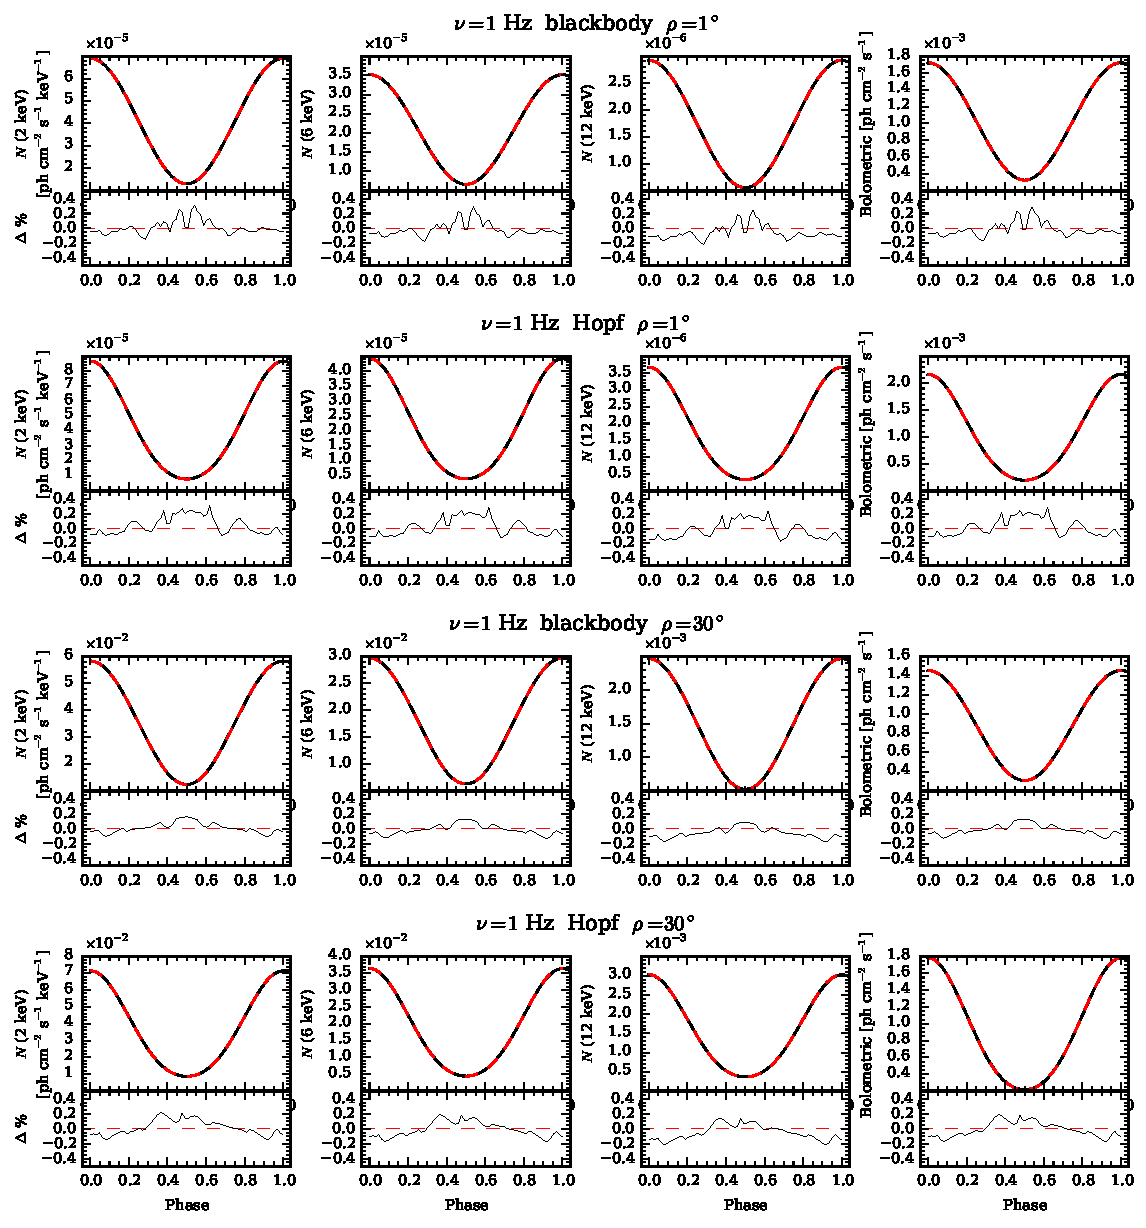
\epsfig{file=jpulsec1.pdf,width=17.0cm}}
\caption{The light curve (monochromatic number flux at 2 keV) comparisons with slowly rotating spherical star ($R = 12$ km, $M = 1.6$ $\msun$, $\nu = 1$ Hz, $i = 60 \degree$, $\theta = 50 \degree$ and $T_{\mathrm{eff}} = 2$ keV) emitting according to blackbody law or Hopf profile with spot size either 1 or 30 degrees. Black solid line shows the pulse profiles computed using the methods described in this Thesis (S+D) and red dashed line is a profile computed with the light-ray tracing methods (LTM). The residuals are shown in the lower panel as $\Delta = (\mathrm{model}_{\mathrm{S+D}}/\mathrm{model}_{\mathrm{LTM}})*100$ \%. Figure from Nättilä and Pihajoki (in preparation).
\label{fig:jpulse1}}
\end{figure}
%%%%%%%%%%%%%%%%%%%%%%%%%%%%%%%%%%%%%%%%%%%%%


%%%%%%%%%%%%%%%%%%%%%%%%%%%%%%%%%%%%%%%%%%%%%
\begin{figure}
\centerline{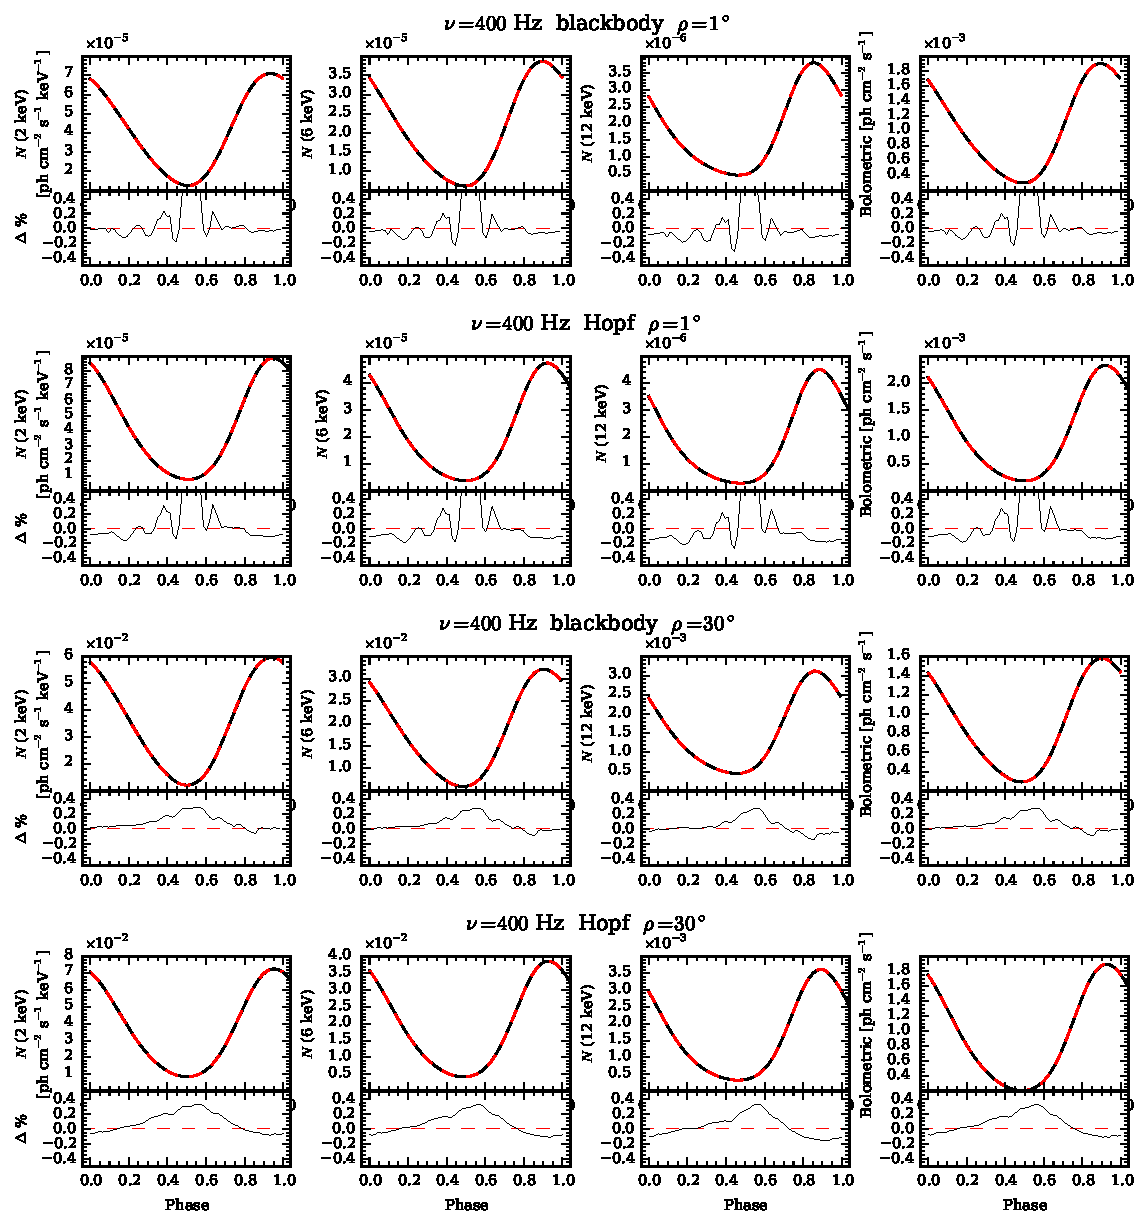
\epsfig{file=jpulsec2.pdf,width=17.0cm}}
\caption{The light curve (monochromatic number flux at 2 keV) comparisons with rapidly rotating spherical star ($\nu = 400$ Hz). Otherwise the parameters and symbols are the same as in figure \ref{fig:jpulse1}. Figure from Nättilä and Pihajoki (in preparation).
\label{fig:jpulse2}}
\end{figure}
%%%%%%%%%%%%%%%%%%%%%%%%%%%%%%%%%%%%%%%%%%%%%


%%%%%%%%%%%%%%%%%%%%%%%%%%%%%%%%%%%%%%%%%%%%%
\begin{figure}
\centerline{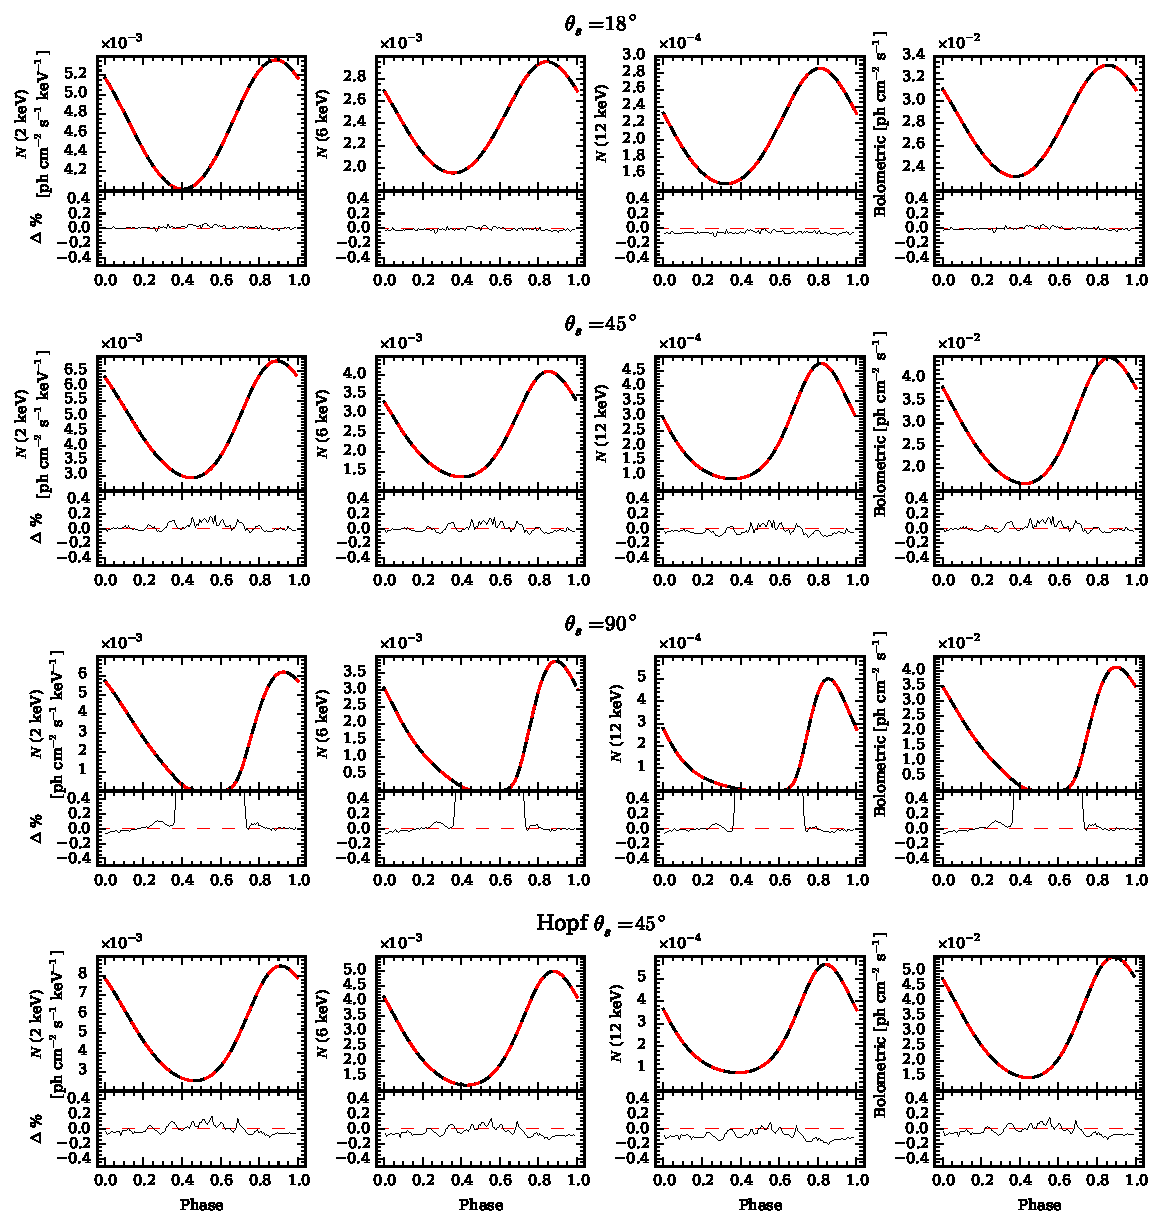
\epsfig{file=jpulsec3.pdf,width=17.0cm}}
\caption{The light curve (monochromatic number flux at 2 keV) comparisons with an oblate star ($R_{\mathrm{eq}} = 12$ km, $M = 1.4$ $\msun$, $\nu = 700$ Hz, $i = 45 \degree$, $\rho = 10 \degree$ and $T_{\mathrm{eff}} = 2$ keV) emitting according to blackbody law or Hopf profile with different spot colatitudes: $\theta$ = 18 $\degree$, 45 $\degree$ and 90 $\degree$. The symbols are the same as in figures \ref{fig:jpulse1} and \ref{fig:jpulse2}. Figure from Nättilä and Pihajoki (in preparation).
\label{fig:jpulse3}}
\end{figure}
%%%%%%%%%%%%%%%%%%%%%%%%%%%%%%%%%%%%%%%%%%%%%




\subsection{Bayesian inference}


%http://math.nyu.edu/~mjlewis/foo.pdf %about Monte Carlo

The model presented in the previous section can be used to constrain parameters of neutron stars by using Bayesian inference. We can fit the observed data to the model and use Markov Chain Monte Carlo (MCMC) methods to integrate over the parameter space to find the most probable values for the parameters of the model \cite{mc_methods_book}. The data can also be synthetic (as in this thesis) in order to test our methods and tools. %if the sampler will actually find the same values that were used when generating the data. 
Previously the constraints of neutron star masses and radii with synthetic data have been studied e.g. by Ka Ho Lo et al, 2013 \cite{miller}. %(for future space missions).   
More about the synthetic data of this thesis is presented in the Results section. 

The aim of this work is to determine the most probable ("best-fit") values of the parameters in the pulse profile model, given the "observed" \ 
waveform, and the confidence regions for the values of these parameters. The goal is also to study the effect of polarization measurements on to the posterior probability distributions. Probabilities are calculated using Bayes' theorem, which is presented in the next section. The standard Metropolis sampling method of the parameter space and a modern ensemble sampler (used in this thesis) are discussed in the following three sections. 

\subsubsection{Bayesian analysis}

We are interested in the probability of the parameters $\textbf{y}$ of the waveform model when the observed waveform is known. The probability distribution of the parameters given the data is $p(\textbf{y}|\mathcal{D})$, where $\mathcal{D}$ is the energy- and oscillation phase-resolved waveform data (synthetic in our case). According to the Bayes' theorem this (posterior) probability distribution can be obtained from the likelihood of the data, given the parameter values as \cite{nattila_bayes}


\be \label{eq:bayes}
p(\textbf{y}|D) \propto p(D|\textbf{y})p(\textbf{y}).
\ee

In the previous equation $p(\mathcal{D}|\textbf{y})$ is the likelihood or the probability distribution of the data given the parameters. The factor $p(\textbf{y})$ is the prior probability distribution of the parameter values. As a first approximation we use uniform prior, which is the most uninformative prior. Later we take in to account the information of polarization measurements and make the priors of inclination and spot colatitude non-uniform to study their impact on the fit. The constant of proportionality is the inverse of the normalization factor, but it is irrelevant when estimating the values of the parameters in a given model. 


\subsubsection{Metropolis-Hastings}

The original standard MCMC algorithm is called the Metropolis algorithm \cite{metropolis53}\cite{hastings70}. %(Metropolis et al., 1953 \cite{metropolis53}; Hastings, 1970 \cite{hastings70}). 
It is a MCMC method for obtaining a sequence of random samples from a probability distribution. It generates these random samples by moving in a random walk; that is in some sequence $X_{1}...X_{t}$. Metropolis algorithm, like all the other MCMC sampling methods, satisfy the so-called Markov property. It means that the conditional probability distribution of $X_{t+1}$, given all the past elements, is independent of all the other states except the previous state \cite{kaiser}:

 \be \label{eq:markov_prop}
P(X_{t+1} = x|X_{t}. . . X_{1}) = P(X_{t+1} = x|X_{t}).
\ee
So generally we can conclude that a Markov chain is a random walk with Markov property.
 
The Metropolis algorithm works by taking an arbitrary move near the current
point in the sequence. If $X_{t}$ is the sample at time t, then the new sample Y is proposed from the proposal distribution $q(Y|X_{t})$. In the original Metropolis algorithm this distribution must be symmetric, meaning that $q(X_{t}|Y)$ = $q(Y|X_{t})$. However, in Metropolis-Hastings algorithm it may be non-symmetric. The likelihood of the new sample is then in both cases compared to that of the previous sample. The likelihood ratio $\alpha$ between the two states is calculated from the following equation \cite{tuomi}:
\be \label{eq:likely_ratio} 
\alpha = \frac{p(Y|\mathcal{D})q(X_{t}|Y)}{p(X_{t}|\mathcal{D})q(Y|X_{t})}.
\ee
The conditional probabilities given the data are calculated using the Bayes formula (\ref{eq:bayes}). The ratio of these probabilities is multiplied with the ratio of proposal distributions (sometimes called transition kernels) so that the algorithm satisfies a detailed balance condition. It is an important property for proving the convergence of the chain. It states that the number of transitions from $X_{t}$ to $Y$ must be the same as from $Y$ to $X_{t}$.  The proposal density $q(X_{t}|Y)$ describes the probability of a transition from $Y$ to $X_{t}$ in the parameter space.

The next step is to decide whether the likelihood ratio is high enough in order to accept the new step. In Metropolis(-Hastings) algorithm, we automatically accept a step, if $\alpha \ge 1$, but otherwise with a probability $\alpha$ (if $\alpha$ is greater than a random number between 0 and 1). If the new state is accepted, we repeat the first steps using now $Y$ as the current point. Otherwise we propose a new sample using again the same $X_{t}$. 


%If the probability distribution function (PDF) has greater value at that point, then the walk always moves there. If the PDF has a smaller value, then the move is accepted with probability dependent on how much less likely.

It may be noticed that the acceptance rule simplifies significantly when the
proposal density is indeed symmetric ($q(X_{t}|Y)$=$q(Y|X_{t})$). The algorithm is typically repeated until the obtained chains are long enough in the sense that their statistics do not change considerably when adding new members to the chain. The statistical representativeness of the sample can be verified
%Whether the obtained samples are statistically representative of the posterior can be verified 
if multiple chains with different initial states result in the same posterior density. It is also necessary to remove the so-called initial warm-up period ("burn-in"), %perhaps tens of thousands of the first iterations ("burn-in"),
since the probability distribution has not yet converged in that case. %those. 
There is no general theory to decide the optimal burn-in period.%for how long burn-on is required.%length of burn-in required. 


\subsubsection{Autocorrelation and difficulties with Metropolis}

Metropolis(-Hastings) algorithm has also some limitations. The samples are not independent (as we would like them to be), since they are generated in a chain (concerns though also other MCMC methods). The correlation between the samples can be measured by the autocorrelation time (also called integrated autocorrelation time) \cite{ensemble1}: 
\be \label{eq:autocorr_time}
\tau = \sum_{t=-\infty}^{\infty} \frac{C(t)}{C(0)} ,
\ee
where the function $C(t)$ is autocovariance with lag t:
\be \label{eq:autocovariance}
C(t) = \lim_{t'\to\infty}\mathrm{Cov}(V(X_{t+t'}),V(X_{t})).
\ee
Here $V(X_{t})$ is an observable. Basically this measures how related the series of numbers $V(X_{t})$ is with itself. 

One way to compute the autocorrelation time is to use the weights (log-likelihoods) of the fits as the observable $V(X_{t})$. If the weights are strongly correlated with many different lags, $\tau$ will be large. Of course most of the correlation is originated from samples close to each other (small lags). This can be seen by inspecting the autocovariance as function of the lag (see Figure \ref{fig:acexample} in Results). There is no way to get completely rid of autocorrelation, but at least some of the problem may be solved by making the sequence of samples thinner. In principle the number of samples which should be independent is $N_{\mathrm{step}}/\tau$, where $N_{\mathrm{step}}$ is the total number of steps \cite{kaiser}. However especially with Metropolis $\tau$ is typically high (unless very carefully designed proposal densities) meaning that very high fraction of the samples should be removed.

One other major disadvantage is that the Metropolis algorithm may work poorly for skewed, or anisotropic, distributions, depending on the proposal distribution. One example of such is a two dimensional skewed probability distribution (shown in figure \ref{fig:skewed})
\be \label{eq:skew} 
f(\vec{x}) = \exp(-\frac{(x_{1}-x_{2})^{2}}{2\epsilon_{c}}-\frac{(x_{1}+x_{2})^{2}}{2}),
\ee
where $\epsilon_{c}$ is a constant. Metropolis (like many other MCMC strategies too) would be forced to make perturbations of order $\sqrt{\epsilon_{c}}$ and would have slow equilibration. A better MCMC sampler would use larger perturbations in (-1,1) than in (1,1) direction. However, the problem gets worse in high dimensions, where it is difficult to tune all the step sizes correctly. As a next step to address this issue we can use the ensemble sampler, which is presented in the next section. 


%%%%%%%%%%%%%%%%%%%%%%%%%%%%%%%%%%%%%%%%%%%%%
\begin{figure}
\centerline{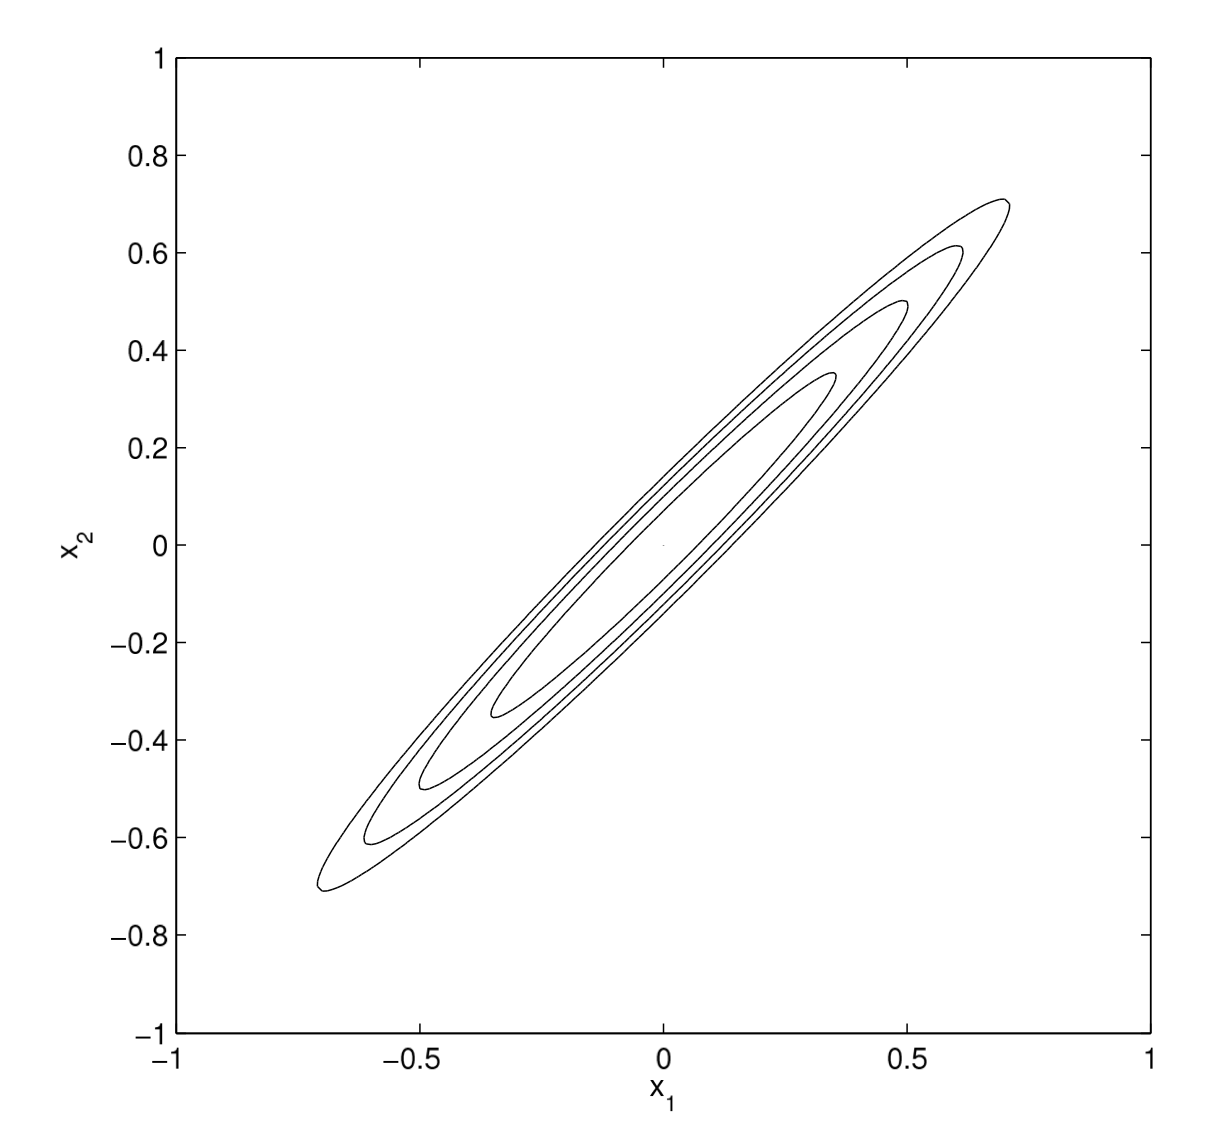
\epsfig{file=skewed.png,width=10.0cm}}
\caption{Contours of the Gaussian density defined in expression (\ref{eq:skew}). Figure 1 from Goodman and Weare (2010) \cite{ensemble1}.
\label{fig:skewed}}
\end{figure}
%%%%%%%%%%%%%%%%%%%%%%%%%%%%%%%%%%%%%%%%%%%%%


\subsubsection{Ensemble sampler}

The affine invariant ensemble sampler is a novel MCMC method developed a few years ago \cite{ensemble1}. %(Goodman and Weare, 2010 \cite{ensemble1}). 
The algorithm has a similar structure to Metropolis scheme, and still uses a proposal and accept/reject step. But instead of only one sequence $X_{1}...X_{t}$, we use now a group or ensemble of sequences. Each member of the group is called a walker. On each iteration the algorithm generates a new sample for every walker using the  current positions of all of the other walkers in
the ensemble. However, each walker is independent of the other walkers. They are correlated only with the previous states of other walkers and their own previous state. After burn-in the distribution of each walker should be converged to the invariant posterior probability distribution.

%each walker is also distributed according to the invariant posterior probability distribution.



%http://msp.org/camcos/2010/5-1/camcos-v5-n1-p04-s.pdf
%https://arxiv.org/pdf/1202.3665v4.pdf


The ensemble sampler is called affine invariant, since its performance is unaffected by affine transformations of space. This means that one can sample a probability distribution function $g(x) = Af(x) + b$ either directly or sample first $f$ and then apply $A$ and $b$ afterwords. 
%sampling a PDF g(x) = Af(x) + b is equivalent to sampling f then applying A and b %after. 
For this reason the algorithm is particularly useful for sampling badly scaled distributions. Computational tests show that the affine invariant methods can be significantly faster than standard MCMC methods on highly skewed distributions.

In the ensemble sampler the  Markov chain is evolved by moving one walker at time. Each walker $X_{k}$ is updated using the current positions of all of the other walkers in
the ensemble. We call them a complementary ensemble. The motivation is that the distribution of the walkers in the complementary ensemble carries useful information about the probability density of the parameters. This way the trial move can be adapted to the target density.  


%If L is the number of the walkers, these walkers (besides $X_{k}$ ) form the complementary ensemble

%\be \label{eq:compl_ensemble} 
%X_{k}(t+1) = X_{1}(t + 1), . . . , X_{k−1}(t + 1), X_{k+1}(t), . . . , X_{l} (t).
%1=2
%\ee

%In this algorithm, we use a group or ensemble of sequences. Each member of
%the ensemble is called a walker.

One of the simplest affine invariant trial moves, and the move we use here, is the so-called stretch-move. In a stretch-move algorithm each walker is moved using only one randomly selected complementary walker (see fig. \ref{fig:smove}). The move of current walker $k$ is proposed along a line between the walker itself and the complementary walker $j$ according to the distribution \cite{emceehammer}
\be \label{eq:smove}
Y = X(j) + Z(X(k)-X(j)),
\ee
where the scaling variable $Z$ satisfies the symmetry condition
\be \label{eq:symmetry_condition}
g(1/z) = zg(z).
\ee
This ensures that the move (\ref{eq:smove}) is symmetric in the usual informal way Metropolis is discussed.% i.e, detailed balance is satisfied.


%%%%%%%%%%%%%%%%%%%%%%%%%%%%%%%%%%%%%%%%%%%%%
\begin{figure}
\centerline{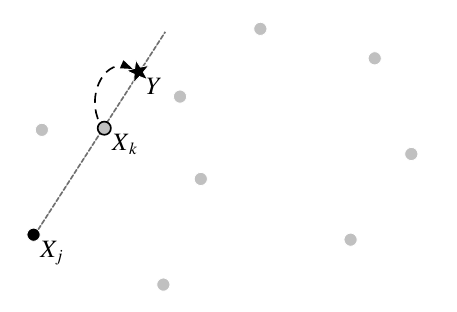
\epsfig{file=stretchmove.png,width=10.0cm}}
\caption{A stretch move for updating the position of $X_{k}$ based on the position of another random walker, $X_{j}$ (subscript identifies here the walker instead of the step count). The light-gray walkers are other members of the ensemble. Figure 2 from Goodman and Weare (2010) \cite{ensemble1}.
\label{fig:smove}}
\end{figure}
%%%%%%%%%%%%%%%%%%%%%%%%%%%%%%%%%%%%%%%%%%%%%


When deciding whether the new sample is accepted or not, the Metropolis-Hastings selection rules are again applied. However, instead of equation (\ref{eq:likely_ratio}) the likelihood ratio is now calculated (for a given walker) as
\be \label{eq:likely_ratio_smove} 
\alpha = Z^{N-1}\frac{p(Y|\mathcal{D})}{p(X_{t}|\mathcal{D})},
\ee
where $N$ is now the number of parameters sampled \cite{emceehammer}. The transition probabilities $q$ are not needed, since in the case of symmetric move (\ref{eq:smove}) the acceptance ratio (\ref{eq:likely_ratio_smove}) can be shown to satisfy the detailed balance condition. 


%=dimension of the parameter space

%\subsubsection{Implementation}

\clearpage

\section{Results}

As mentioned earlier the aim of this work is to determine the probability distributions of the parameters in the pulse profile model (especially the mass and radius), given the synthetic pulse profile, and study the effects of polarization measurements to the results. Some details of the data, sampling and constraints obtained are presented in the three following sections. 


\subsection{Synthetic data}

The synthetic data in this work is made to resemble the real observations as closely as possible. The X-ray count data from \source \ is used as a reference. The amplitude of the modulation in the normalized number fluxes have been set close to the same value in the synthetic data as in the observations. We also use the same energy intervals and same number of phase points as in the real data. The original data is shown in Figure \ref{fig:saxdata}.  

%%%%%%%%%%%%%%%%%%%%%%%%%%%%%%%%%%%%%%%%%%%%%
\begin{figure}
\centerline{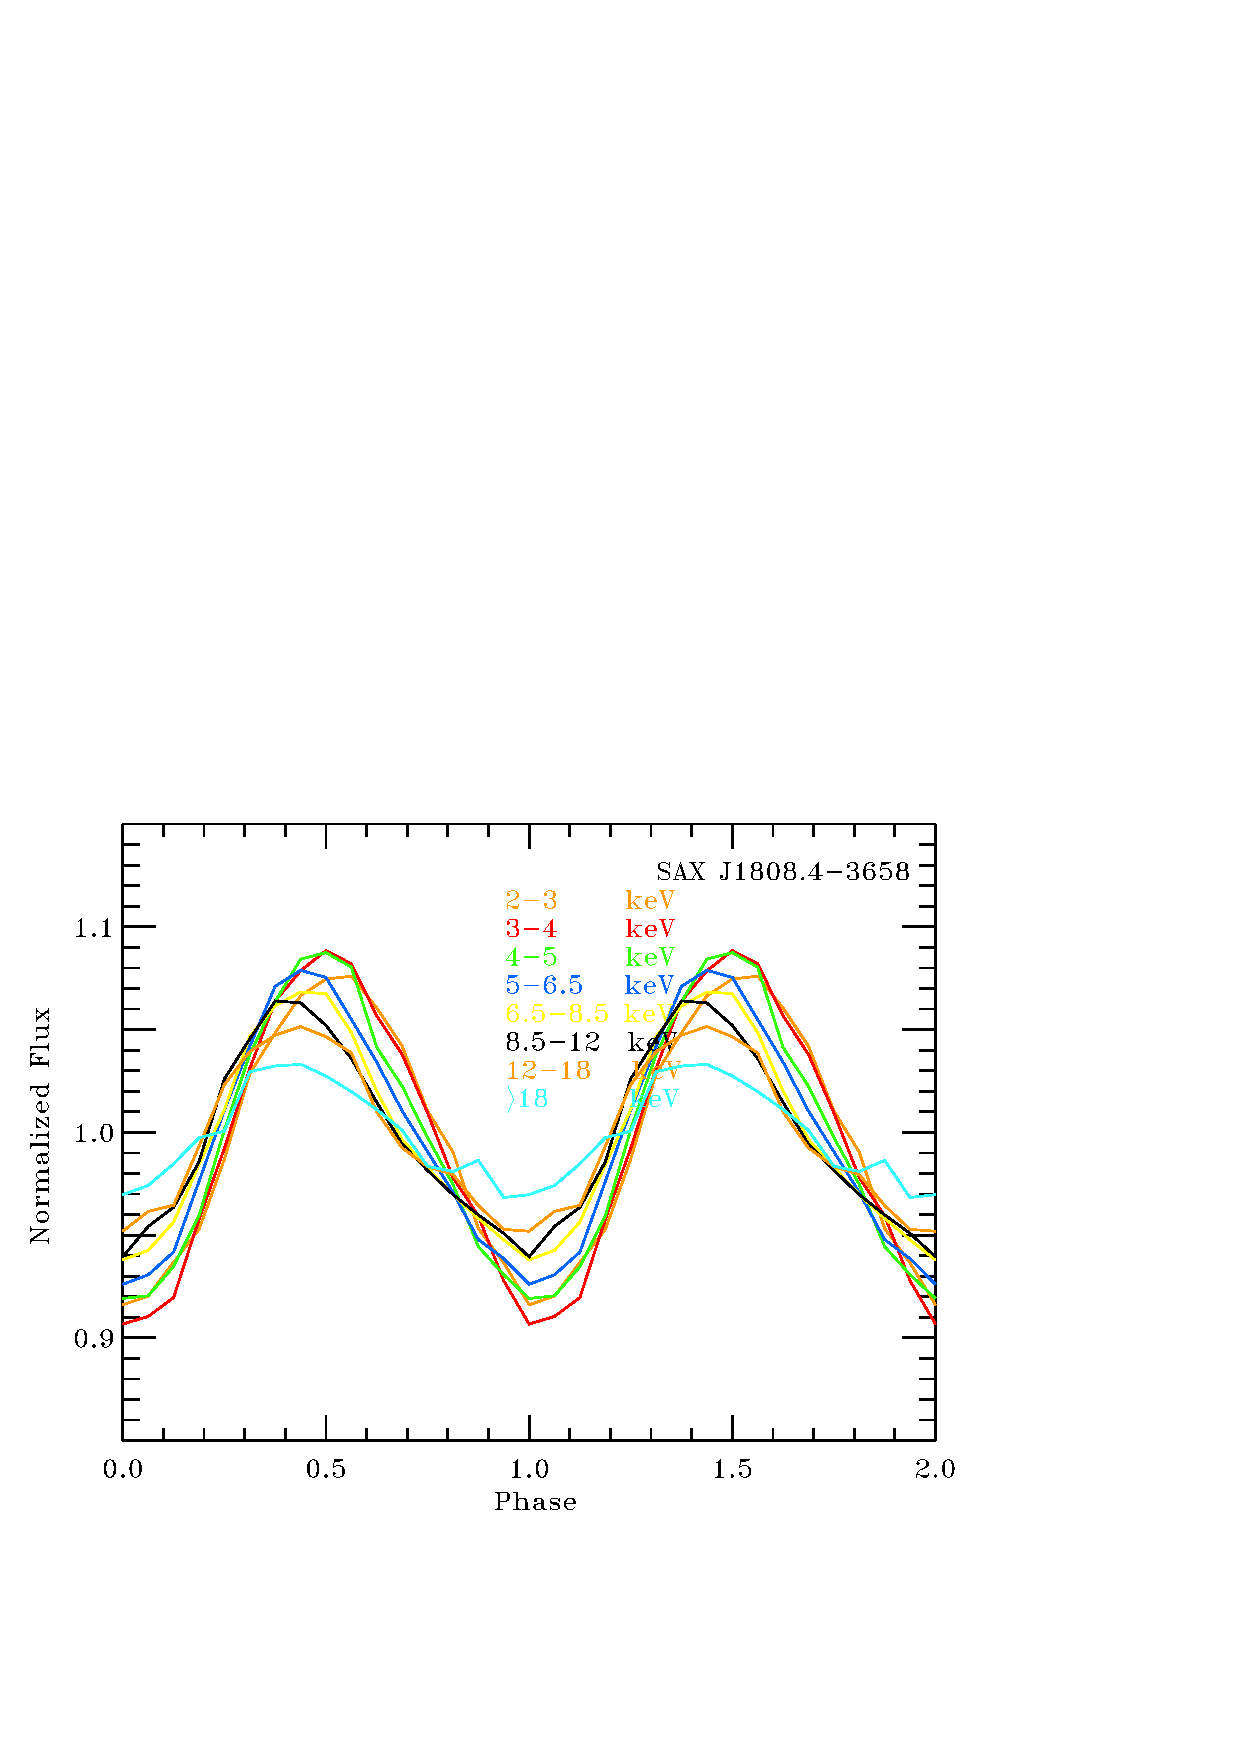
\epsfig{file=data_sax1808.pdf,width=12.0cm}} 
\caption{Normalized number fluxes at different energies as a function of the phase from \source \ measured with RXTE . 
\label{fig:saxdata}}
\end{figure}
%%%%%%%%%%%%%%%%%%%%%%%%%%%%%%%%%%%%%%%%%%%%%


The parameters of the pulse profile model are chosen such that their values are physically reasonable and they produce a light curve similar to the SAX-data. The physical parameters are given in the Table \ref{table:params}. The observed variability amplitude (see equation \ref{eq:amplitude}) is then obtained by choosing inclination $i$ and the colatitude of the spot $\theta$ appropriately, since the amplitude can be approximated (neglecting the Doppler effect and using the Beloborodov's approximation \cite{poutaviironen})
\be \label{eq:amplitude_incthet}
A \approx \frac{(1-\rg/R)\sin i \sin \theta}{\rg/R+(1-\rg/R)\cos i \cos \theta}.
\ee 

We see that $i$ and $\theta$ can be changed in the equation (\ref{eq:amplitude_incthet}) without affecting the amplitude. The exact calculation shows also only a small difference between these two parameters. Thus we have created two identical synthetic datasets which differ only in $i$ and $\theta$. We call them datasets for polar and equatorial spots even though the spots are not exactly at the pole or equator. 

The datasets have been generated using our pulse profile model. Since the observed data always includes noise, we want to have it also in our synthetic data. For this reason a different random number, from a normal distribution with mean equal to zero, is added to the original flux at each phase point. The average size of this random number have been chosen to match closely the known errors of the \source \ data. Thus a relatively larger noise has been added to the highest energy channels, where the count rates are lowest. The normalized synthetic spectral fluxes and their errors (amount of noise added) are shown in the Figures (\ref{fig:syntpol2}) and (\ref{fig:synteq2}).


%They have been created using the pulse profile model and adding random Gaussian noise %to the fluxes for every phase point. A larger noise was added to the highest energy %channels. 



In our simulations we see how the two datasets with different $i-\theta$ solutions can be separated from each other at least with help of the polarization information giving constraints to $i$ to $\theta$. We also show their effect on the constraints of mass and radius, which are our parameters of interest. 




\begin{center}
\begin{table}
  \caption{Paramters of the synthetic datasets.}
\label{table:params}
\begin{center}
  \begin{tabular}{| c | c |}
    \hline
     Parameter & Value\\ \hline
      Radius $R$ & 12.0 km  \\ \hline
      Mass $M$ & 1.5 $\msun$  \\ \hline
      Inclination $i$ & 5 $\degree$ or 75 $\degree$ \\ \hline
      Spot colatitude $\theta$ & 75 $\degree$ or 5 $\degree$ \\ \hline
      Spot angular size $\rho$ & 10.0 $\degree$  \\ \hline
      Distance $D$ & 2.5 kpc \\ \hline
      Temperature $T_{\mathrm{eff}}$ & 2.0 keV \\

    \hline
  \end{tabular}
  \end{center} 

  \end{table}
\end{center} 



%



%%%%%%%%%%%%%%%%%%%%%%%%%%%%%%%%%%%%%%%%%%%%%
\begin{figure}
\centerline{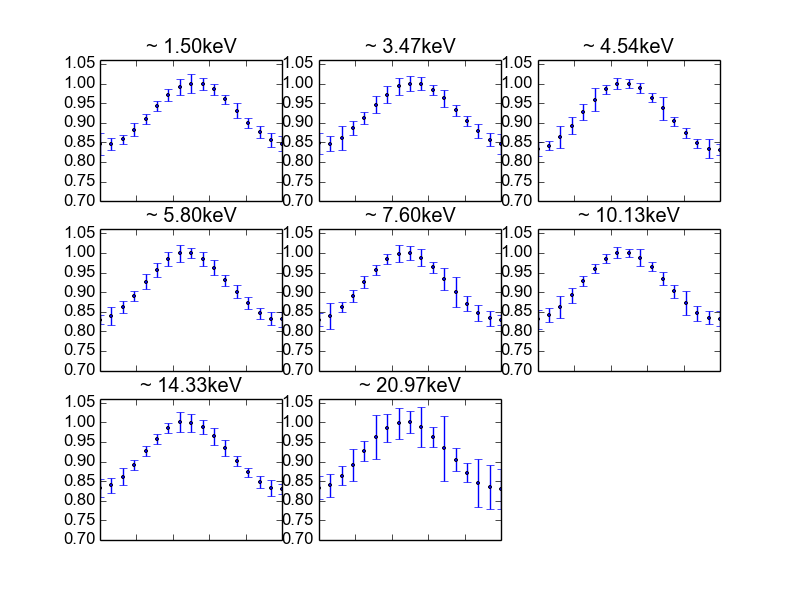
\epsfig{file=synt_sax_pol2.png,width=17.0cm}}
\caption{Synthetic data: Normalized number fluxes as a function of the phase at different energies for $i = 75 \deg$ and $\theta = 5 \deg$. The phase is from 0 to 1. Other parameters are shown in the Table \ref{table:params}.
\label{fig:syntpol2}}
\end{figure}
%%%%%%%%%%%%%%%%%%%%%%%%%%%%%%%%%%%%%%%%%%%%%


%%%%%%%%%%%%%%%%%%%%%%%%%%%%%%%%%%%%%%%%%%%%%
\begin{figure}
\centerline{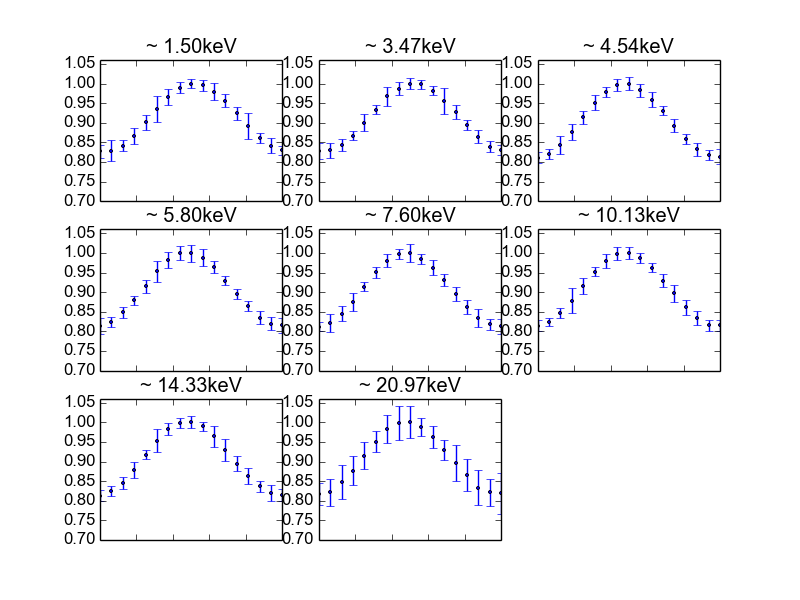
\epsfig{file=synt_sax_eq2.png,width=17.0cm}}
\caption{Synthetic data: Normalized number fluxes as a function of the phase at different energies for $i = 5 \deg$ and $\theta = 75 \deg$. The phase is from 0 to 1. Other parameters are shown in the Table \ref{table:params}.
\label{fig:synteq2}}
\end{figure}
%%%%%%%%%%%%%%%%%%%%%%%%%%%%%%%%%%%%%%%%%%%%%


\subsection{Sampling methods}

All the parameters presented in the Table \ref{table:params} except temperature, are sampled using the ensemble sampler. There are also other parameters in the model, which are not currently sampled. %(at least not in this work yet). 
"Beaming parameter" \ is set to zero, meaning that the intensity from the spot does not depend on the emission angle (isotropic beaming). 

We also use only one spherically symmetric hot spot. The oblate shape of the star is described by the function in equation (\ref{rtheta2}). Some parameters affecting the accuracy of the pulse profile calculation have been changed after creating the synthetic data in order to get faster sampling. For example the quadratic interpolation of light bending angles have been replaced by linear interpolation. The accuracy is still more than enough for our purposes. 

To exploit all possible computational power we have also made the ensemble sampler code to run parallel. In this thesis we did simultaneously six independent simulations on six different processors and then combined the results of each individual chain. Thus each processor had its own ensemble (or also called the chain). The number of walkers was set to 20 in each ensemble. 
 
The choice of the reference radius $r_{\mathrm{ref}}$ needed in time delay calculation affects only the phase shift of the waveform. Since we want to simulate a realistic situation where the phase shift is unknown, we use different $r_{\mathrm{ref}}$ in the generation of the data than in the fitting procedure of the ensemble sampler.  

The likelihood of the data for each sample ($p(\mathcal{D}|\textbf{y})$ in equation \ref{eq:bayes}) is calculated by fitting the data to the pulse profile model. To be more specific, we assume that the probability density of the data fluxes $F_{\mathrm{data}}$ given the modeled fluxes $F_{\mathrm{model}}$  is normally distributed around the $F_{\mathrm{model}}$ with the known errors as standard deviation ($\sigma_{\mathrm{E}}$ in the following equation): 
\be \label{eq:gaussprob}
p(F_{\mathrm{data}}|F_{\mathrm{model}}) \propto \exp (\frac{-(F_{\mathrm{data}}-F_{\mathrm{model}})^{2}}{2\sigma_{\mathrm{E}}^{2}}).
\ee
Normalization is not needed, since it will cancel out when calculating likelihood ratios. The total probability density of the data given the sample is the multiplication of $p(F_{\mathrm{data}}|F_{\mathrm{model}})$ from each phase point and at each energy (or the sum of log-probabilities). 

Of course we also need to take in account that we have different phase shift in the data and in the model. For that reason we calculate the model with 5 times higher phase resolution than the model. We calculate the probability densities using equation (\ref{eq:gaussprob}) with different phase shifts in order to marginalize over the uncertainty of phase shift. % using all the possible different phase shifts by shifting the values of fluxes in a correct way. 
The total probability $p(\mathcal{D}|\textbf{y})$ (which will be used to calculate the likelihood ratio given by equation \ref{eq:likely_ratio_smove}) is the marginalized probability over all phase shifts. 

As a first step we assume that all the prior probabilities of the parameters ($p(\textbf{y})$) are uniform, so that equations (\ref{eq:bayes}) and (\ref{eq:likely_ratio_smove}) give 
\be \label{eq:alpha1}
\alpha = Z^{N-1}\frac{p(D|Y)}{p(D|X_{t})}.
\ee

As a second step we make the prior probabilities of inclination and spot colatitude non-uniform, so that the previous likelihood ratio is multiplied with the ratio of the prior probabilities, to yield
\be \label{eq:alpha2}
\alpha = Z^{N-1}\frac{p(D|Y)p(Y)}{p(D|X_{t})p(X_{t})}.
\ee

It is not obvious what kind of prior probabilities one should use. It depends on how informative constraints we are able to get from the observations to the given parameter. Unlike in the case of the usual flux, the measured polarization differ significantly if $i$ and $\theta$ are switched \cite{poutaviironen}. Thus from modeling the polarization we can get the prior probability distributions to these parameters. In this thesis we choose to use normally distributed prior probabilities of $i$ and $\theta$ around $0 \degree$ or $90 \degree$ to study the effect on the posterior probabilities of mass and radius. The standard deviations for these priors are chosen to be $15 \degree$. 

Other prior probabilities of the parameters are kept always uniform inside their sampling intervals. The sizes of these intervals are the same as the sizes of the corresponding axes in the posterior probability Figures in the next section. 



\subsection{Parameter constraints}

%%%%%%%%%%%%%%%%%%%%%%%%%%%%%%%%%%%%%%%%%%%%%
\begin{figure}
\centerline{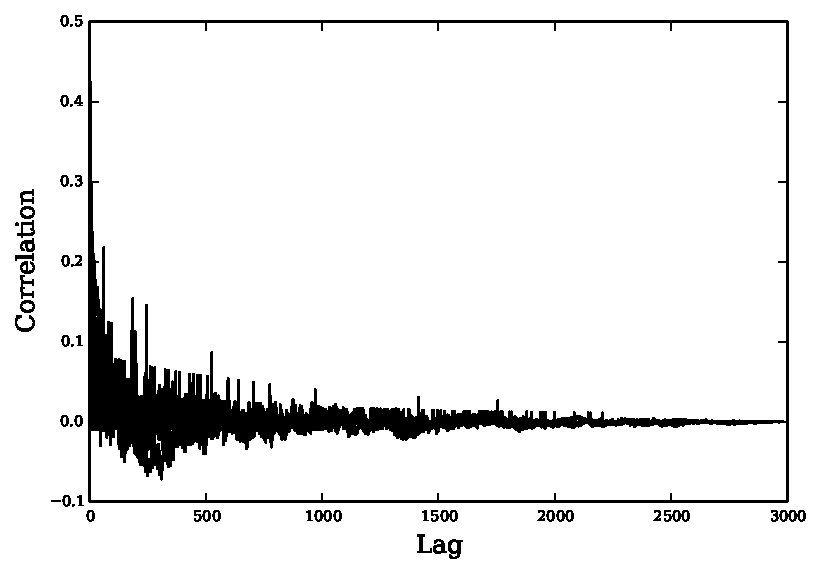
\epsfig{file=ac_fpol.pdf,width=12.0cm}}
\caption{Autocorrelations of the all the ensembles of the polar spot with only uniform priors.
\label{fig:acexample}}
\end{figure}
%%%%%%%%%%%%%%%%%%%%%%%%%%%%%%%%%%%%%%%%%%%%%


%%%%%%%%%%%%%%%%%%%%%%%%%%%%%%%%%%%%%%%%%%%%%
\begin{figure}
\centerline{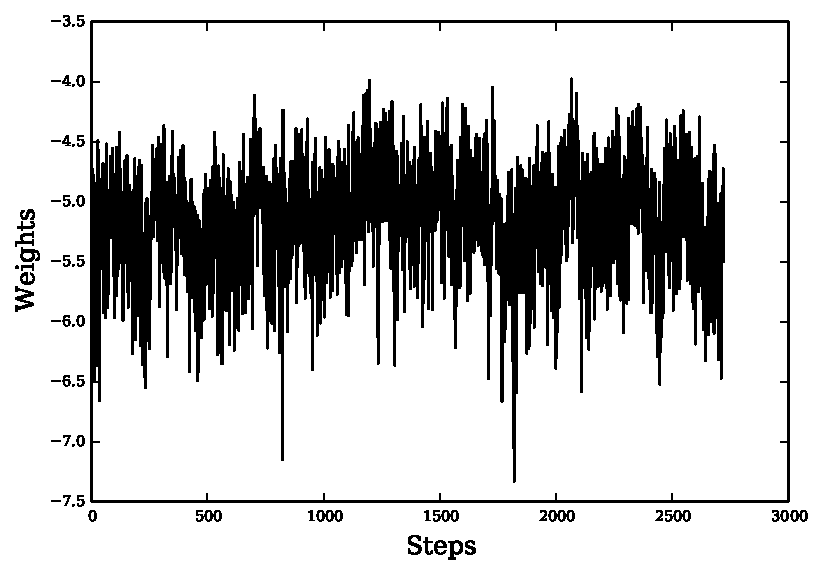
\epsfig{file=weights_example.pdf,width=12.0cm}}
\caption{Log-likelihoods after the burn-in is removed in one ensemble.
\label{fig:wexample}}
\end{figure}
%%%%%%%%%%%%%%%%%%%%%%%%%%%%%%%%%%%%%%%%%%%%%

Before obtaining the final posterior probability distributions we have reduced the burn-in phase from each ensemble by removing the first 20 000 samples from each chain. After that we still have approximately 50 000 samples left belonging to each ensemble.  Figure (\ref{fig:wexample}) shows one example of the log-likelihoods of a converged chain in one of the simulations. In that Figure we use an averaged step of ensemble, which is an average of 20 (number of walkers in the ensemble) consecutive single accepted steps. However for many ensembles we found few walkers which didn't seem to achieve convergence even after a long time (they appeared as sharp peaks in the log-likelihood plots).

The same averaged steps are also used in Figure \ref{fig:acexample}, where we show an example of the autocorrelation. The autocorrelations of all the six ensembles from one simulation are presented using the weights as observables (see equation \ref{eq:autocovariance}). The Figure shows the autocorrelation only approximatively, since one should make sure that the ensemble averaged weights are calculated for walkers being at a same state of their sequence. We may however see that in general the correlation is not very strong, and we have reduced it by taking every fifth sample from the chain.%... Thinning we used is .... (TBD)  

The results of our samplings are presented in the Figures \ref{fig:polpost}-\ref{fig:eqpostpr}. From these posterior probability distributions we can easily see how the prior information of angles $\theta$ and $i$ improves the fits of the mass and radius of the neutron star (by comparing Figures \ref{fig:polpostpr} and \ref{fig:polpost} or Figures \ref{fig:eqpostpr} and \ref{fig:eqpost}). 

Without the prior information we get the highest probabilities for the lowest masses and radii, since those correspond to more possible solutions in  $\theta$ and $i$ than the highest masses and radii. In this case we are only able to get upper limits to the mass and radius. The polar and equatorial spots give very similar results compared to each other as excepted (Figures \ref{fig:polpost} and \ref{fig:eqpost}). However they are not identical, which shows that switching $\theta$ and $i$ has a significant (but not very large) effect on the light curves of the pulsar. It seems also slightly easier to find the correct $\theta$-$i$ solution  in the case of the equatorial spot (although in the one-dimensional histograms the small angles give always a higher peak in the probability density because of the marginalization and the shape of two-dimensional distribution of $\theta$-$i$). 

In case of non-uniform priors for $\theta$ and $i$ (Figures \ref{fig:polpostpr} and \ref{fig:eqpostpr}) we find the correct solutions for $\theta$ and $i$ even though our prior distributions are not centered  around the correct values. The posterior probability distributions for the mass and radius are now also distributed on both sides of the correct values having the maximum near the correct value. Most importantly both the lower and upper limits can now be determined. 

The angular size of the spot $\rho$ is found to be the closest to the correct value of all the  parameters in our sampling. The highest probability is very close to $10 \degree$, which is the value used when creating the datasets. Partly this is due to the choice to sample the distance in a quite small interval (between 2 and 3 kpc). For that reason the size of the spot cannot change very much in order to keep the observed count rate at a correct level. 



%%%%%%%%%%%%%%%%%%%%%%%%%%%%%%%%%%%%%%%%%%%%%
\begin{figure}
\centerline{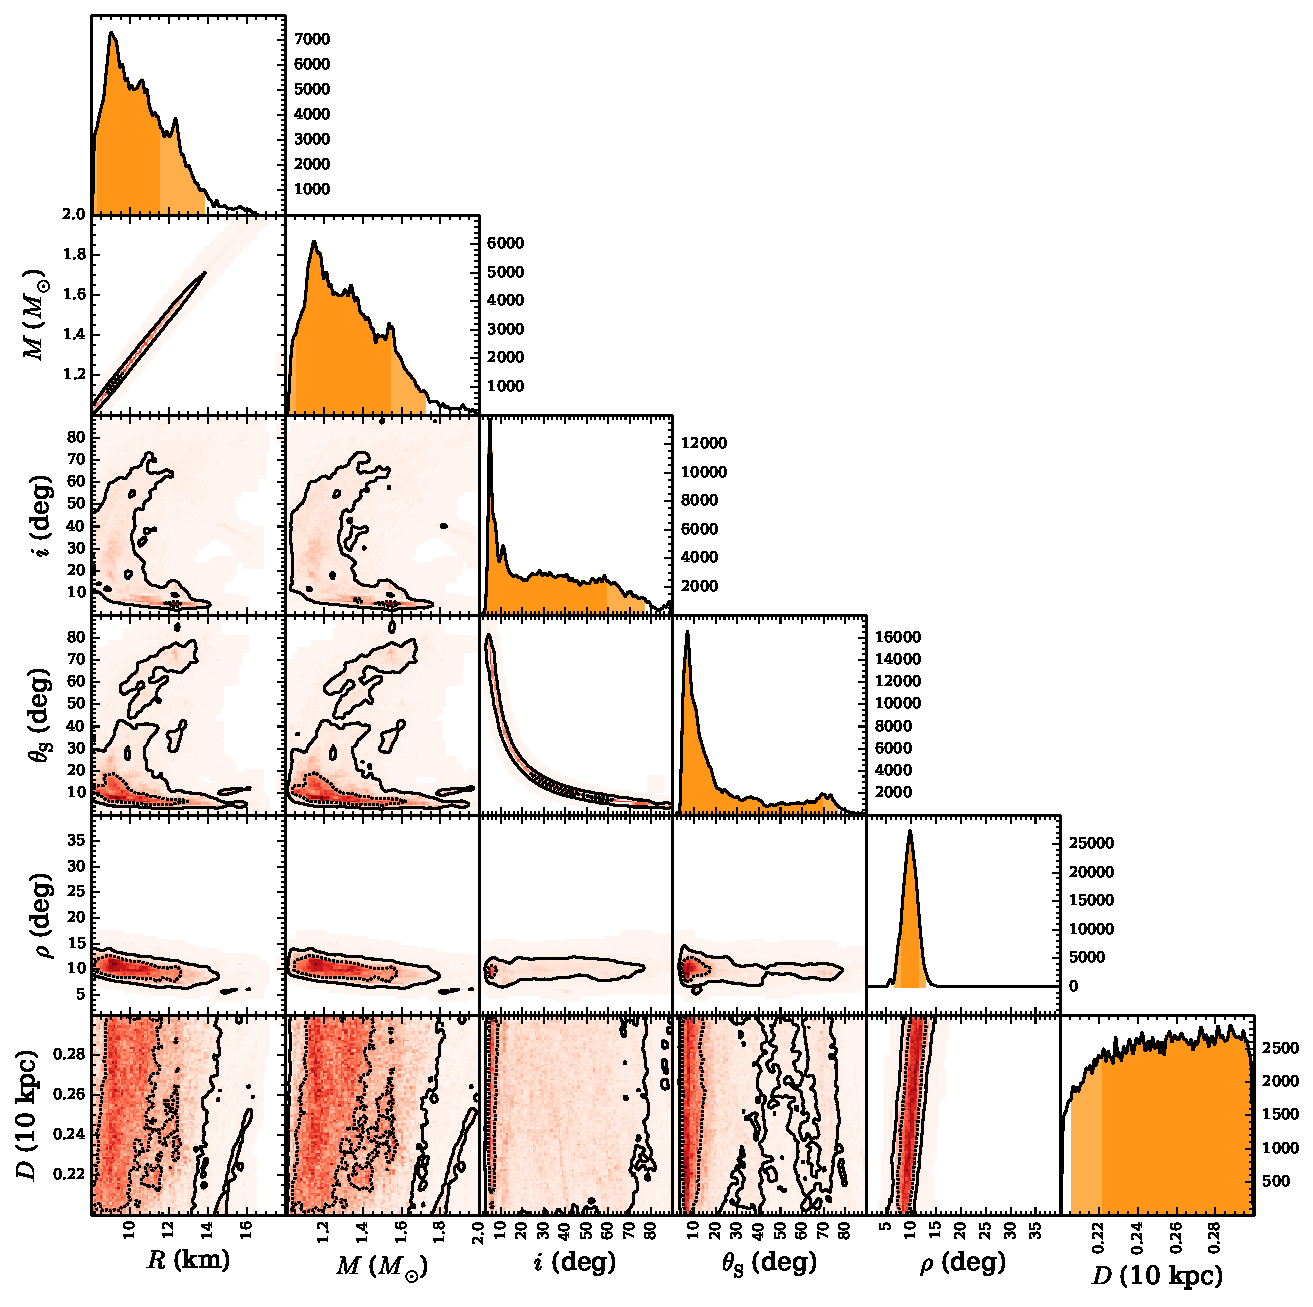
\epsfig{file=fpol.pdf,width=17.0cm}}
\caption{Posterior probability distributions of radius $R$, mass $m$, observer inclination $i$, spot colatitude $\theta_{s}$, spot angular size $\rho$ and distance $D$ for the polar spot with only uniform priors. The one-dimensional distributions are normalized to give 1 as the total probability. The dark orange color shows a one $\sigma_{E}$ and the light orange color a two $\sigma_{E}$ credibility interval. In the 2D posterior distributions the solid contour shows a 95 \% and the dashed contour a 68 \% credibility region.  
\label{fig:polpost}}
\end{figure}
%%%%%%%%%%%%%%%%%%%%%%%%%%%%%%%%%%%%%%%%%%%%%

%%%%%%%%%%%%%%%%%%%%%%%%%%%%%%%%%%%%%%%%%%%%%
\begin{figure}
\centerline{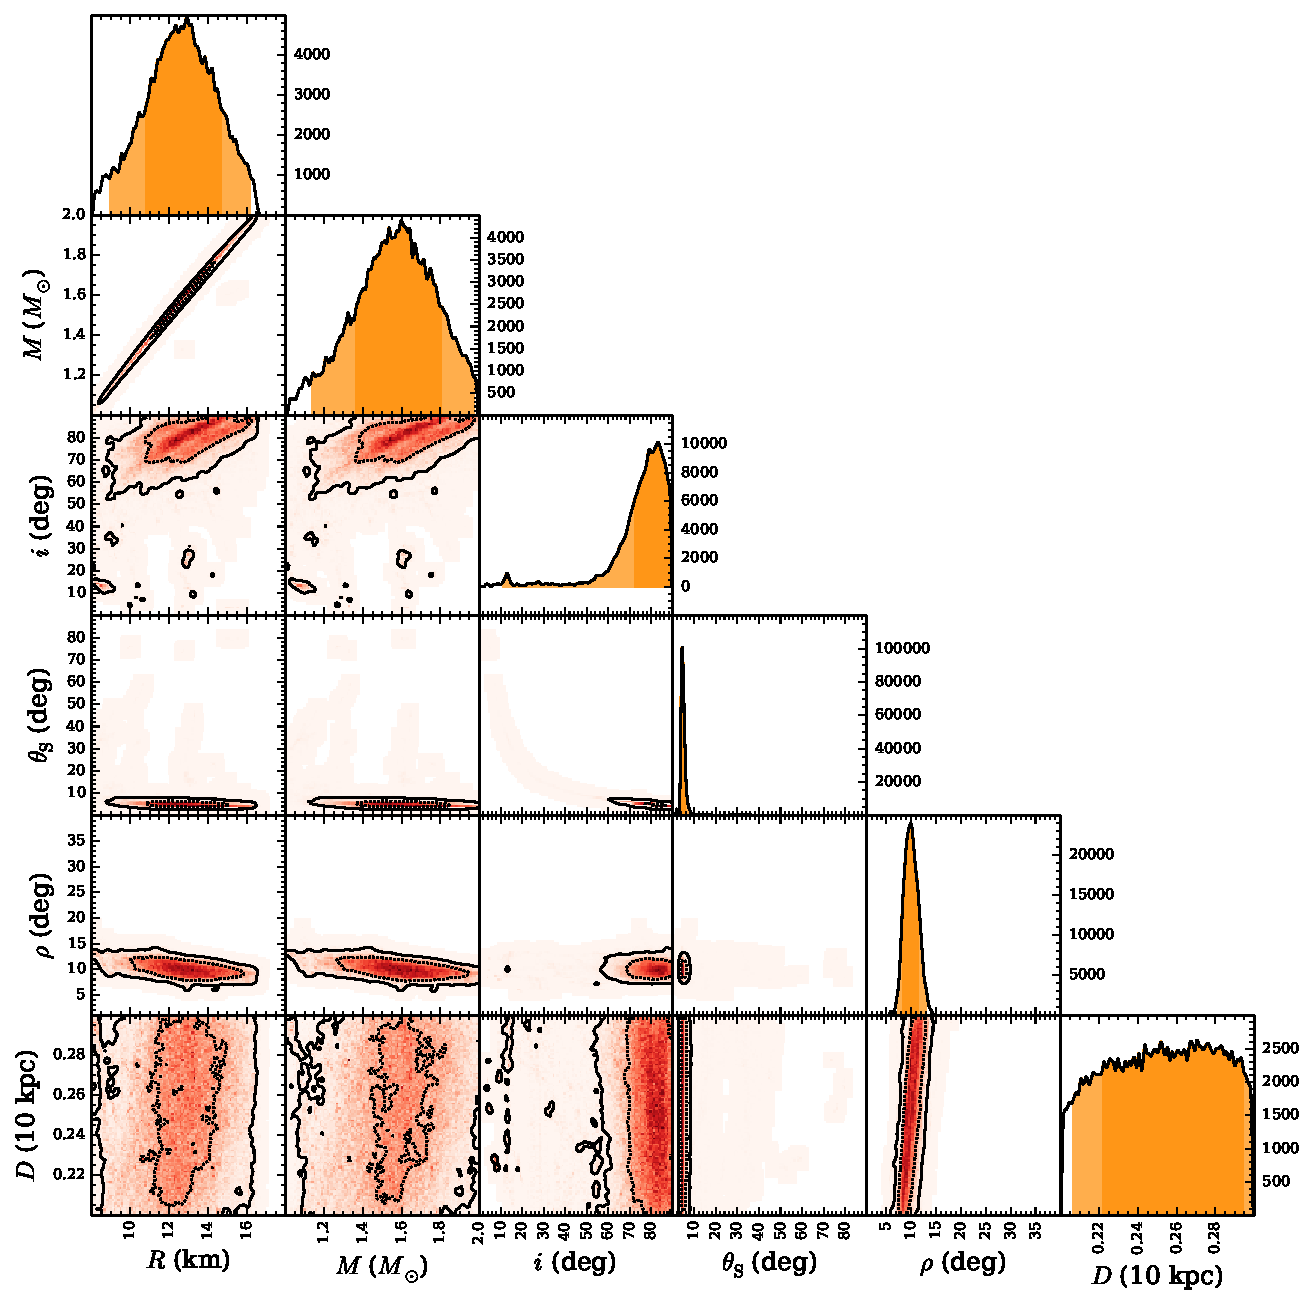
\epsfig{file=fpolpr.pdf,width=17.0cm}}
\caption{Posterior probability distributions of radius $R$, mass $m$, observer inclination $i$, spot colatitude $\theta_{s}$, spot angular size $\rho$ and distance $D$ for the polar spot with non-uniform $i$ and $\theta$ priors (shown with a blue line). The one-dimensional distributions are normalized to give 1 as the total probability. The dark orange color shows a one $\sigma_{E}$ and the light orange color a two $\sigma_{E}$ credibility interval. In the 2D posterior distributions the solid contour shows a 95 \% and the dashed contour a 68 \% credibility region.
\label{fig:polpostpr}}
\end{figure}
%%%%%%%%%%%%%%%%%%%%%%%%%%%%%%%%%%%%%%%%%%%%%



%%%%%%%%%%%%%%%%%%%%%%%%%%%%%%%%%%%%%%%%%%%%%
\begin{figure}
\centerline{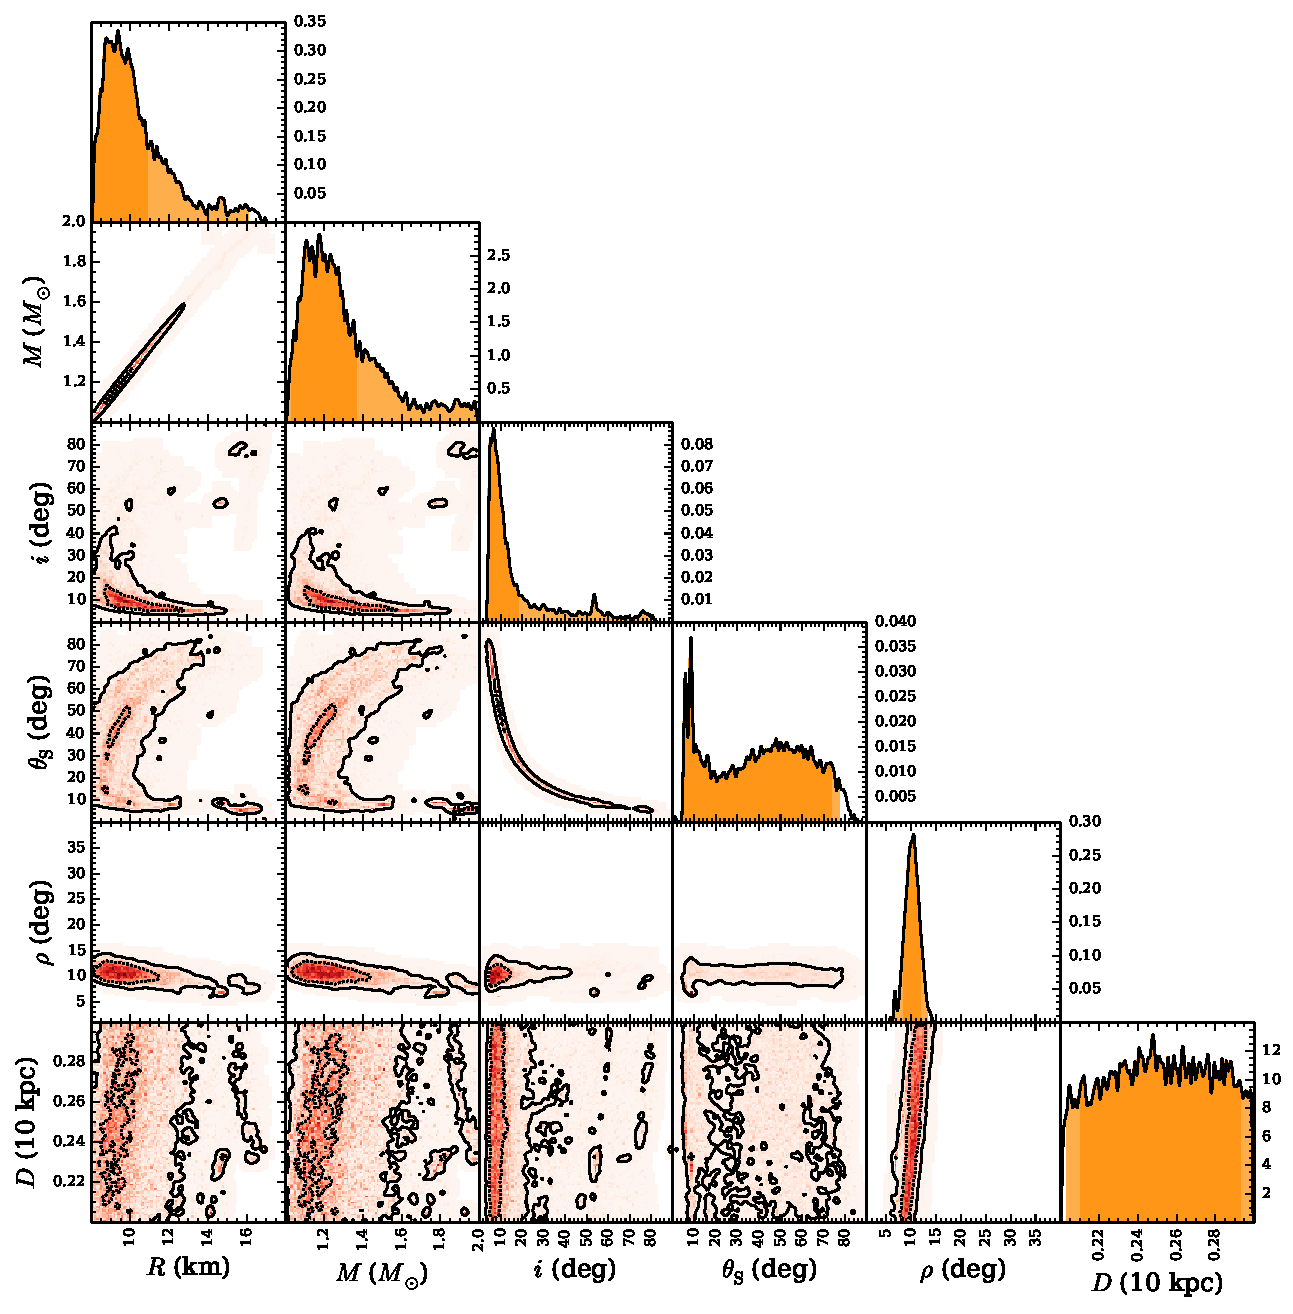
\epsfig{file=feq.pdf,width=17.0cm}}
\caption{Posterior probability distributions of radius $R$, mass $m$, observer inclination $i$, spot colatitude $\theta_{s}$, spot angular size $\rho$ and distance $D$ for the equatorial spot with only uniform priors.The one-dimensional distributions are normalized to give 1 as the total probability. The dark orange color shows a one $\sigma_{E}$ and the light orange color a two $\sigma_{E}$ credibility interval. In the 2D posterior distributions the solid contour shows a 95 \% and the dashed contour a 68 \% credibility region.
\label{fig:eqpost}}
\end{figure}
%%%%%%%%%%%%%%%%%%%%%%%%%%%%%%%%%%%%%%%%%%%%%



%%%%%%%%%%%%%%%%%%%%%%%%%%%%%%%%%%%%%%%%%%%%%
\begin{figure}
\centerline{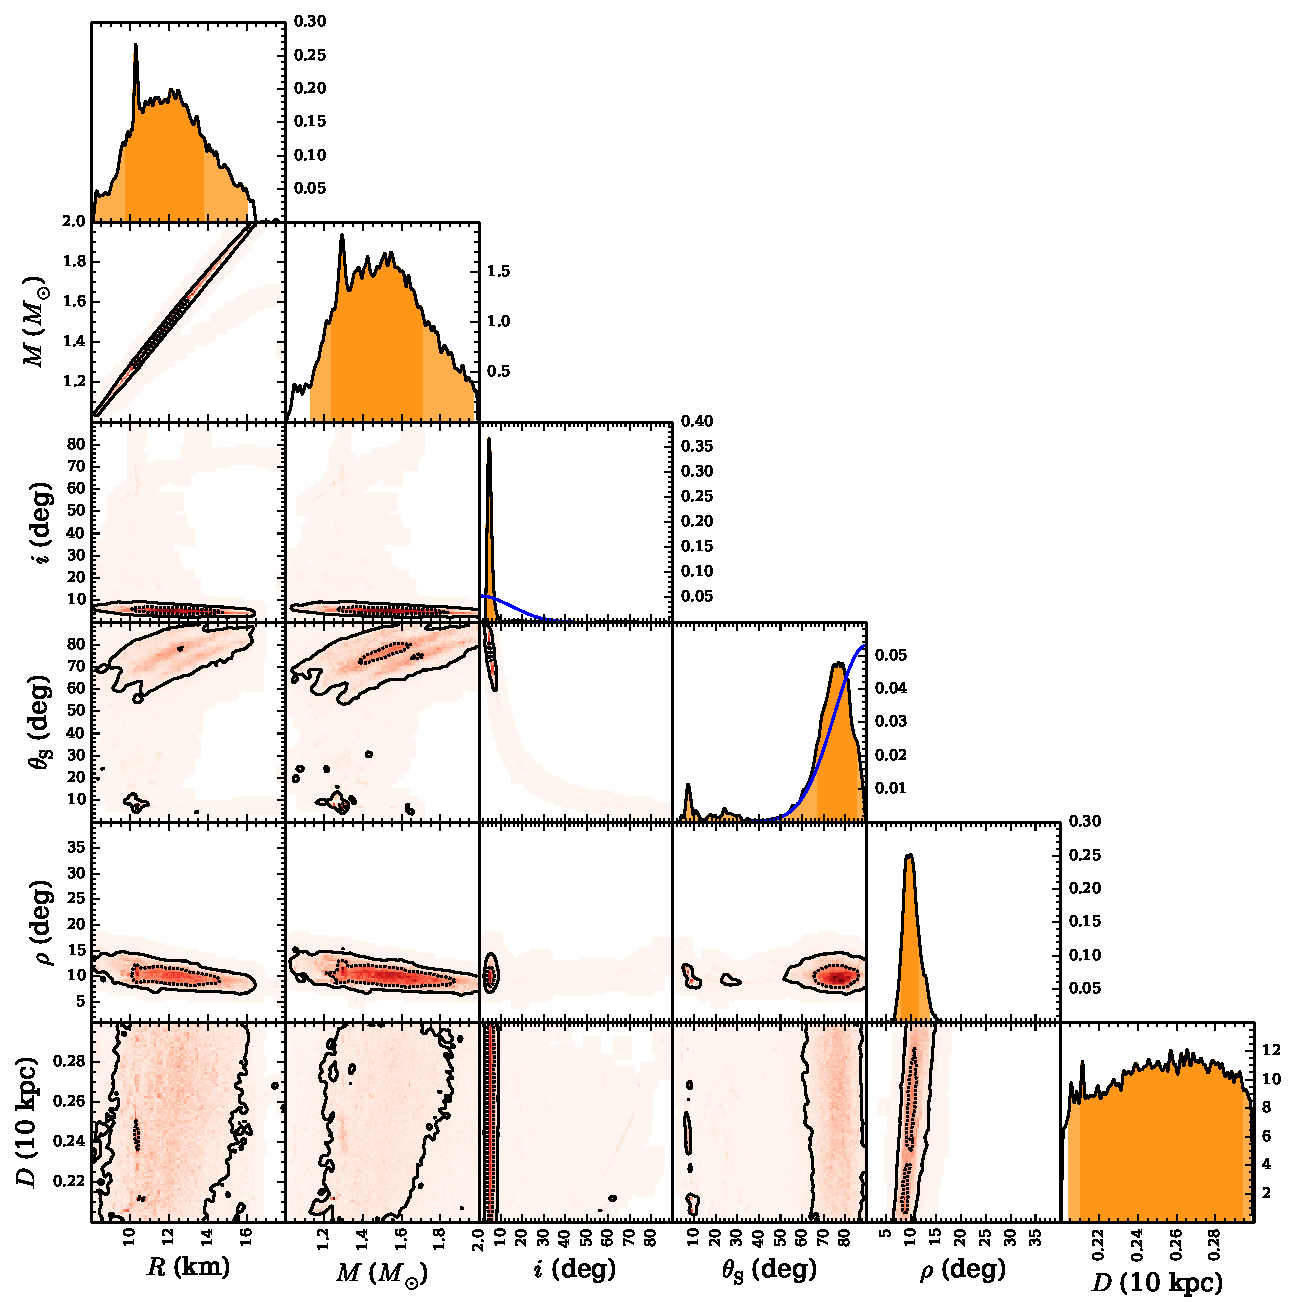
\epsfig{file=feqpr.pdf,width=17.0cm}}
\caption{Posterior probability distributions of radius $R$, mass $m$, observer inclination $i$, spot colatitude $\theta_{s}$, spot angular size $\rho$ and distance $D$ for the equatorial spot with non-uniform $i$ and $\theta$ priors (shown with a blue line). The one-dimensional distributions are normalized to give 1 as the total probability. The dark orange color shows a one $\sigma_{E}$ and the light orange color a two $\sigma_{E}$ credibility interval. In the 2D posterior distributions the solid contour shows a 95 \% and the dashed contour a 68 \% credibility region.
\label{fig:eqpostpr}}
\end{figure}
%%%%%%%%%%%%%%%%%%%%%%%%%%%%%%%%%%%%%%%%%%%%%



\clearpage


\section{Summary and Conclusions}










\iffalse
%esimerkki kuvan liittämisestä
\begin{figure}
\begin{center}
\setlength{\unitlength}{1cm}
\begin{picture}(6,6)(-3,-3)
\put(-1.5,0){\vector(1,0){3}}
\put(2.7,-0.1){$\chi$}
\put(0,-1.5){\vector(0,1){3}}
\multiput(-2.5,1)(0.4,0){13}
{\line(1,0){0.2}}
\multiput(-2.5,-1)(0.4,0){13}
{\line(1,0){0.2}}
\put(0.2,1.4)
{$\beta=v/c=\tanh\chi$}
\qbezier(0,0)(0.8853,0.8853)
(2,0.9640)
\qbezier(0,0)(-0.8853,-0.8853)
(-2,-0.9640)
%\put(-3,-2){\circle*{0.2}}
\end{picture}
%\includegraphics[width=10cm]{kuva.eps}
\caption{Tässä on hieno kuva}
\label{kuva1}
\end{center}
\end{figure}
\fi


%\newpage
%% Rivinväli pienemmäksi viiteluettelossa. Fonttia on vaihdettava, jotta käsky
%% toimisi !
%\renewcommand{\baselinestretch}{1}\large\normalsize
%%
%\begin{thebibliography}{50}% Viiteluettelo. TÄTÄ ON PAKKO KÄYTTÄÄ !
%% Jaa, ai miksi ? No, koska tällä tavalla se on vaan niin pirusti
%% helpompaa.
%\bibitem{lshort} T. Oetiker, H. Partl, I. Hyna and E. Schlegl,
%Not so short introduction to \LaTeX 2e, 1998
%\end{thebibliography}

%
% Vaihtoehtoisesti thebibliography ympäristölle voi käyttää BibTeX
% tietokantaa, jonka voit luoda tai käyttää olemassaolevaa (esim.
% Wihurilla). Suosittelemme tätä lämpimästi!
%
% Bibtex-tietokannan saa helposti tehtyä esim TeXMakerilla. Sitten
% vaan ajetaan latex gradu, bibtex gradu, latex gradu ja latex
% gradu. Ja TADAA viitteet ovat oikeassa järjestyksessä.
%
%\bibliography{/var/bib/yhdistetty}
%\bibliographystyle{wihuri}
%



\newpage
\renewcommand{\baselinestretch}{1}\large\normalsize
%kirjallisuusluettelo
\addcontentsline{toc}{section}{\refname} %Sisällysluetteloon näkymään "Viitteet" sivunumerolla kuten kaikki muukin
%\renewcommand{\baselinestretch}{1.2}\large\normalsize % jos on paljon viitteitä, tällä saa hieman sivuja karsittua
\bibliography{bib1} %Bibtex-tiedoston nimi, joka sijaitsee samassa hakemistossa muiden kanssa. Näitä voi olla useita.
\bibliographystyle{wihuri} %Tyylitiedosto "wihuri.bst". Hieman muutettu alkuperäisestä wihuri-versiosta.

%------------------------
%Jos sulle tulee liitteitä, niin tässä yksi tapa

%\newpage
%\setcounter{page}{1} %nollataan sivulaskurit tai ykköstetään ;)
%\setcounter{section}{0} % sama temppu kappalenumeroille

%\renewcommand\thesection{\Alph{section}} %Kappalenumerointi tyyliin A,B,C...
%\renewcommand\thepage{\Alph{section}-\arabic{page}} % ja sivunumerot %vastaavasti A-1, A-2, B-1...





\end{document} % Se oli siinä !
